\section{Diseño del controlador}

Para controlar la planta a lazo cerrado, se utilizará como modelo base un controlador PID. Este controlador, en tiempo continuo, tiene la siguiente forma
\[
    C(s) = k_p + k_i \frac{1}{s} + k_d s.
\]
En particular, se implmentarán a partir de la expresión anterior un controlador proporcional (tipo P, donde solo $k_p$ es no nulo), proporcional-integral (tipo PI, con $k_d = 0$), y proporcional-derivativo (tipo PD, con $k_i = 0$).

Dado que el controlador será implementado en forma discreta, con $T_s = \qty{20}{\ms}$, se utilizará la siguiente expresión bilineal, donde se reemplaza $s = (z - 1)/(T_s z)$ y se busca una relación de recurrencia en función de la señal error:
\begin{align}
    \label{eq:pid-u}
    u_{k} = k_{p}e_{k} + k_{i}\left(I_{k-1} + \frac{T}{2}e_{k} + \frac{T}{2}e_{k-1}\right) + k_{d}\left(2\frac{e_{k} - e_{k-1}}{T} - D_{k-1}\right),
\end{align}
en donde
\begin{align}
    \label{eq:pid-id}
    I_{k} = I_{k-1} + \frac{T}{2}e_{k} + \frac{T}{2}e_{k-1} && D_{k} = 2\frac{e_{k} - e_{k-1}}{T} - D_{k-1}.
\end{align}

\subsection{Controlador P}

El primer control implementado fue un controlador proporcional, para el cual se aplicaron las Ecuaciones~\eqref{eq:pid-u} y~\eqref{eq:pid-id}, utilizando
\begin{align*}
    K_p = -150, && K_i = 0, && K_d = 0.
\end{align*}

\subsubsection{Rechazo a perturbaciones tipo impulso}

La Figura~\ref{fig:p-pert-salida} muestra la salida de la planta ---la posición del carrito--- real y simulada, ante una perturbación tipo impulso, con el lazo cerrado por el controlador P y una referencia nula (punto de equilibrio).

Se observa que inicialmente hay una concordancia buena entre el modelo y la planta real. Ambos sistemas presentan una oscilación, pero el sistema real se ve severamente afectado por el rozamiento, por lo que llega a estado estacionario tras solo unos segundos. El sistema simulado continúa oscilando durante más tiempo.

\begin{figure}[!tbp]
    \centering
    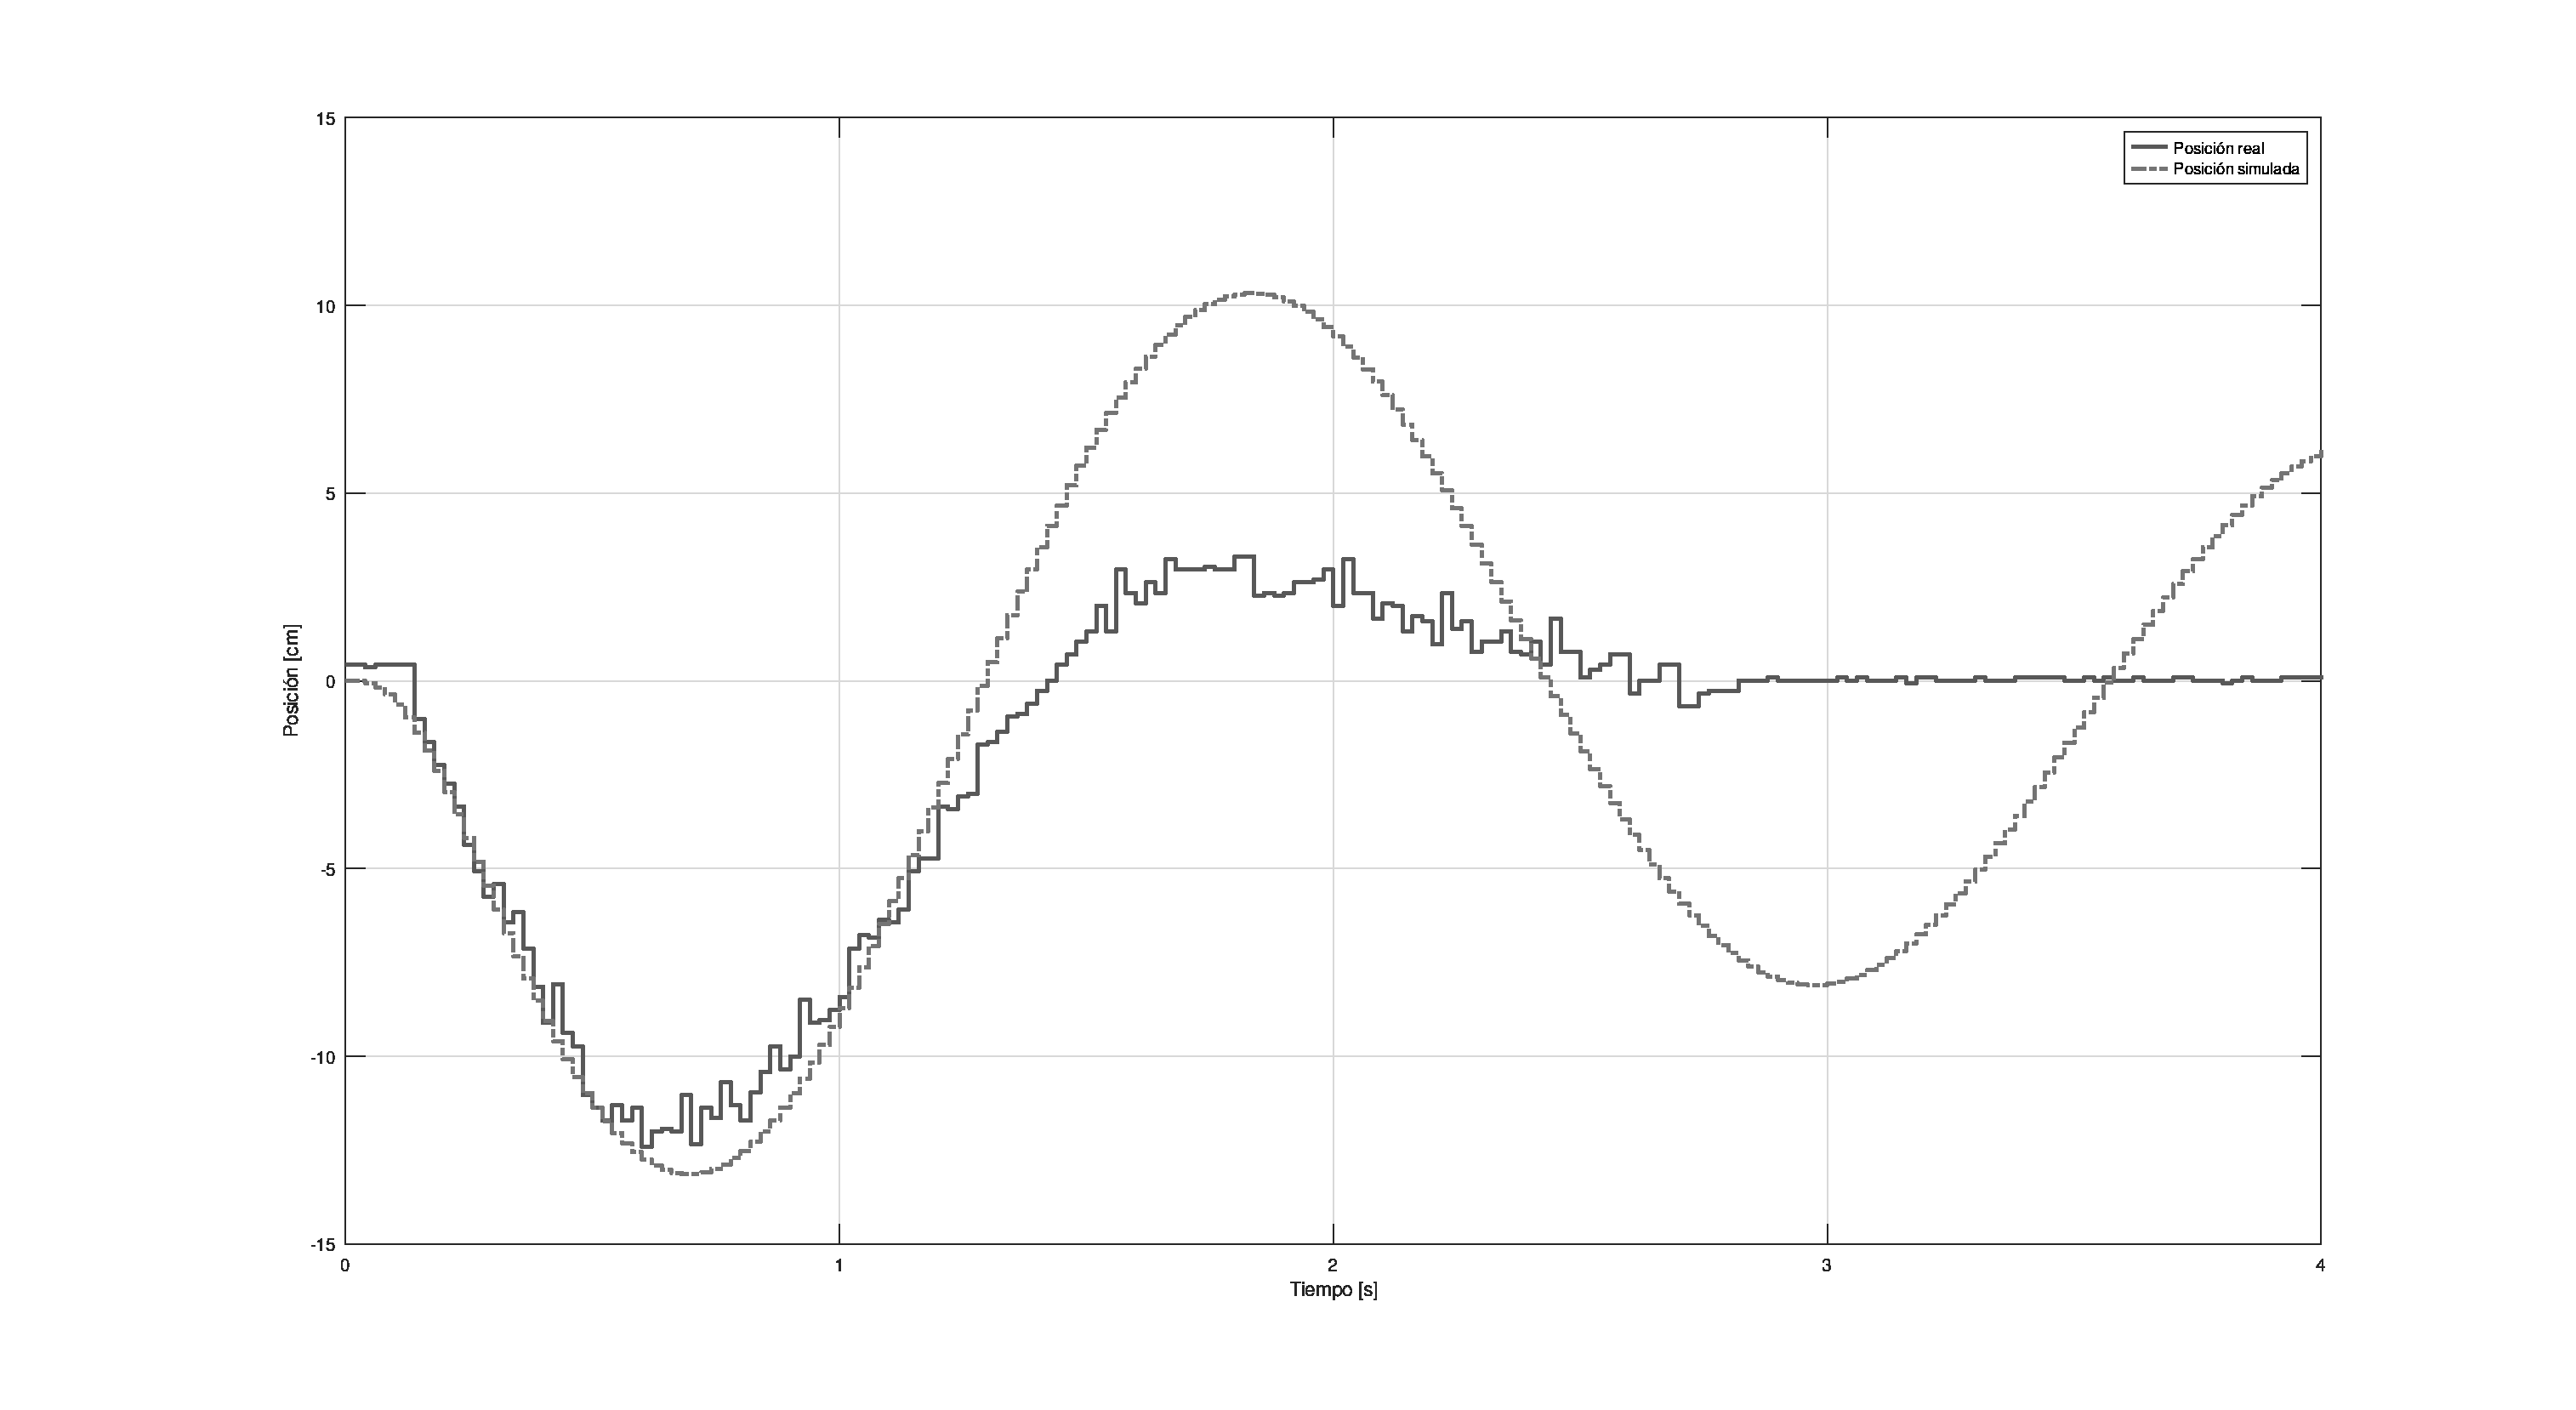
\includegraphics[width=\linewidth]{img/p-pert-salida.eps}
    \caption{Salida del sistema real y simulado ante una perturbación tipo impulso, y un lazo cerrado con un controlador tipo P. Notar que las salidas se escalaron para estar en centímetros.}
    \label{fig:p-pert-salida}
\end{figure}

La Figura~\ref{fig:p-pert-cont} muestra la acción de control ---el comando enviado al servomotor--- real y simulada, ante una perturbación tipo impulso, con el lazo cerrado por el controlador P y una referencia nula (punto de equilibrio). Observar que la acción de control en ningún caso satura los límites impuestos anteriormente. También notar que la forma de onda es la misma que la de la salida (Figura~\ref{fig:p-pert-salida}) salvo un factor de escala, ya que $u = k_p (r - y) = -k_p y$ (y recordar que $k_p < 0$, por lo que $u$ e $y$ tendrán la misma fase).

\begin{figure}[!tbp]
    \centering
    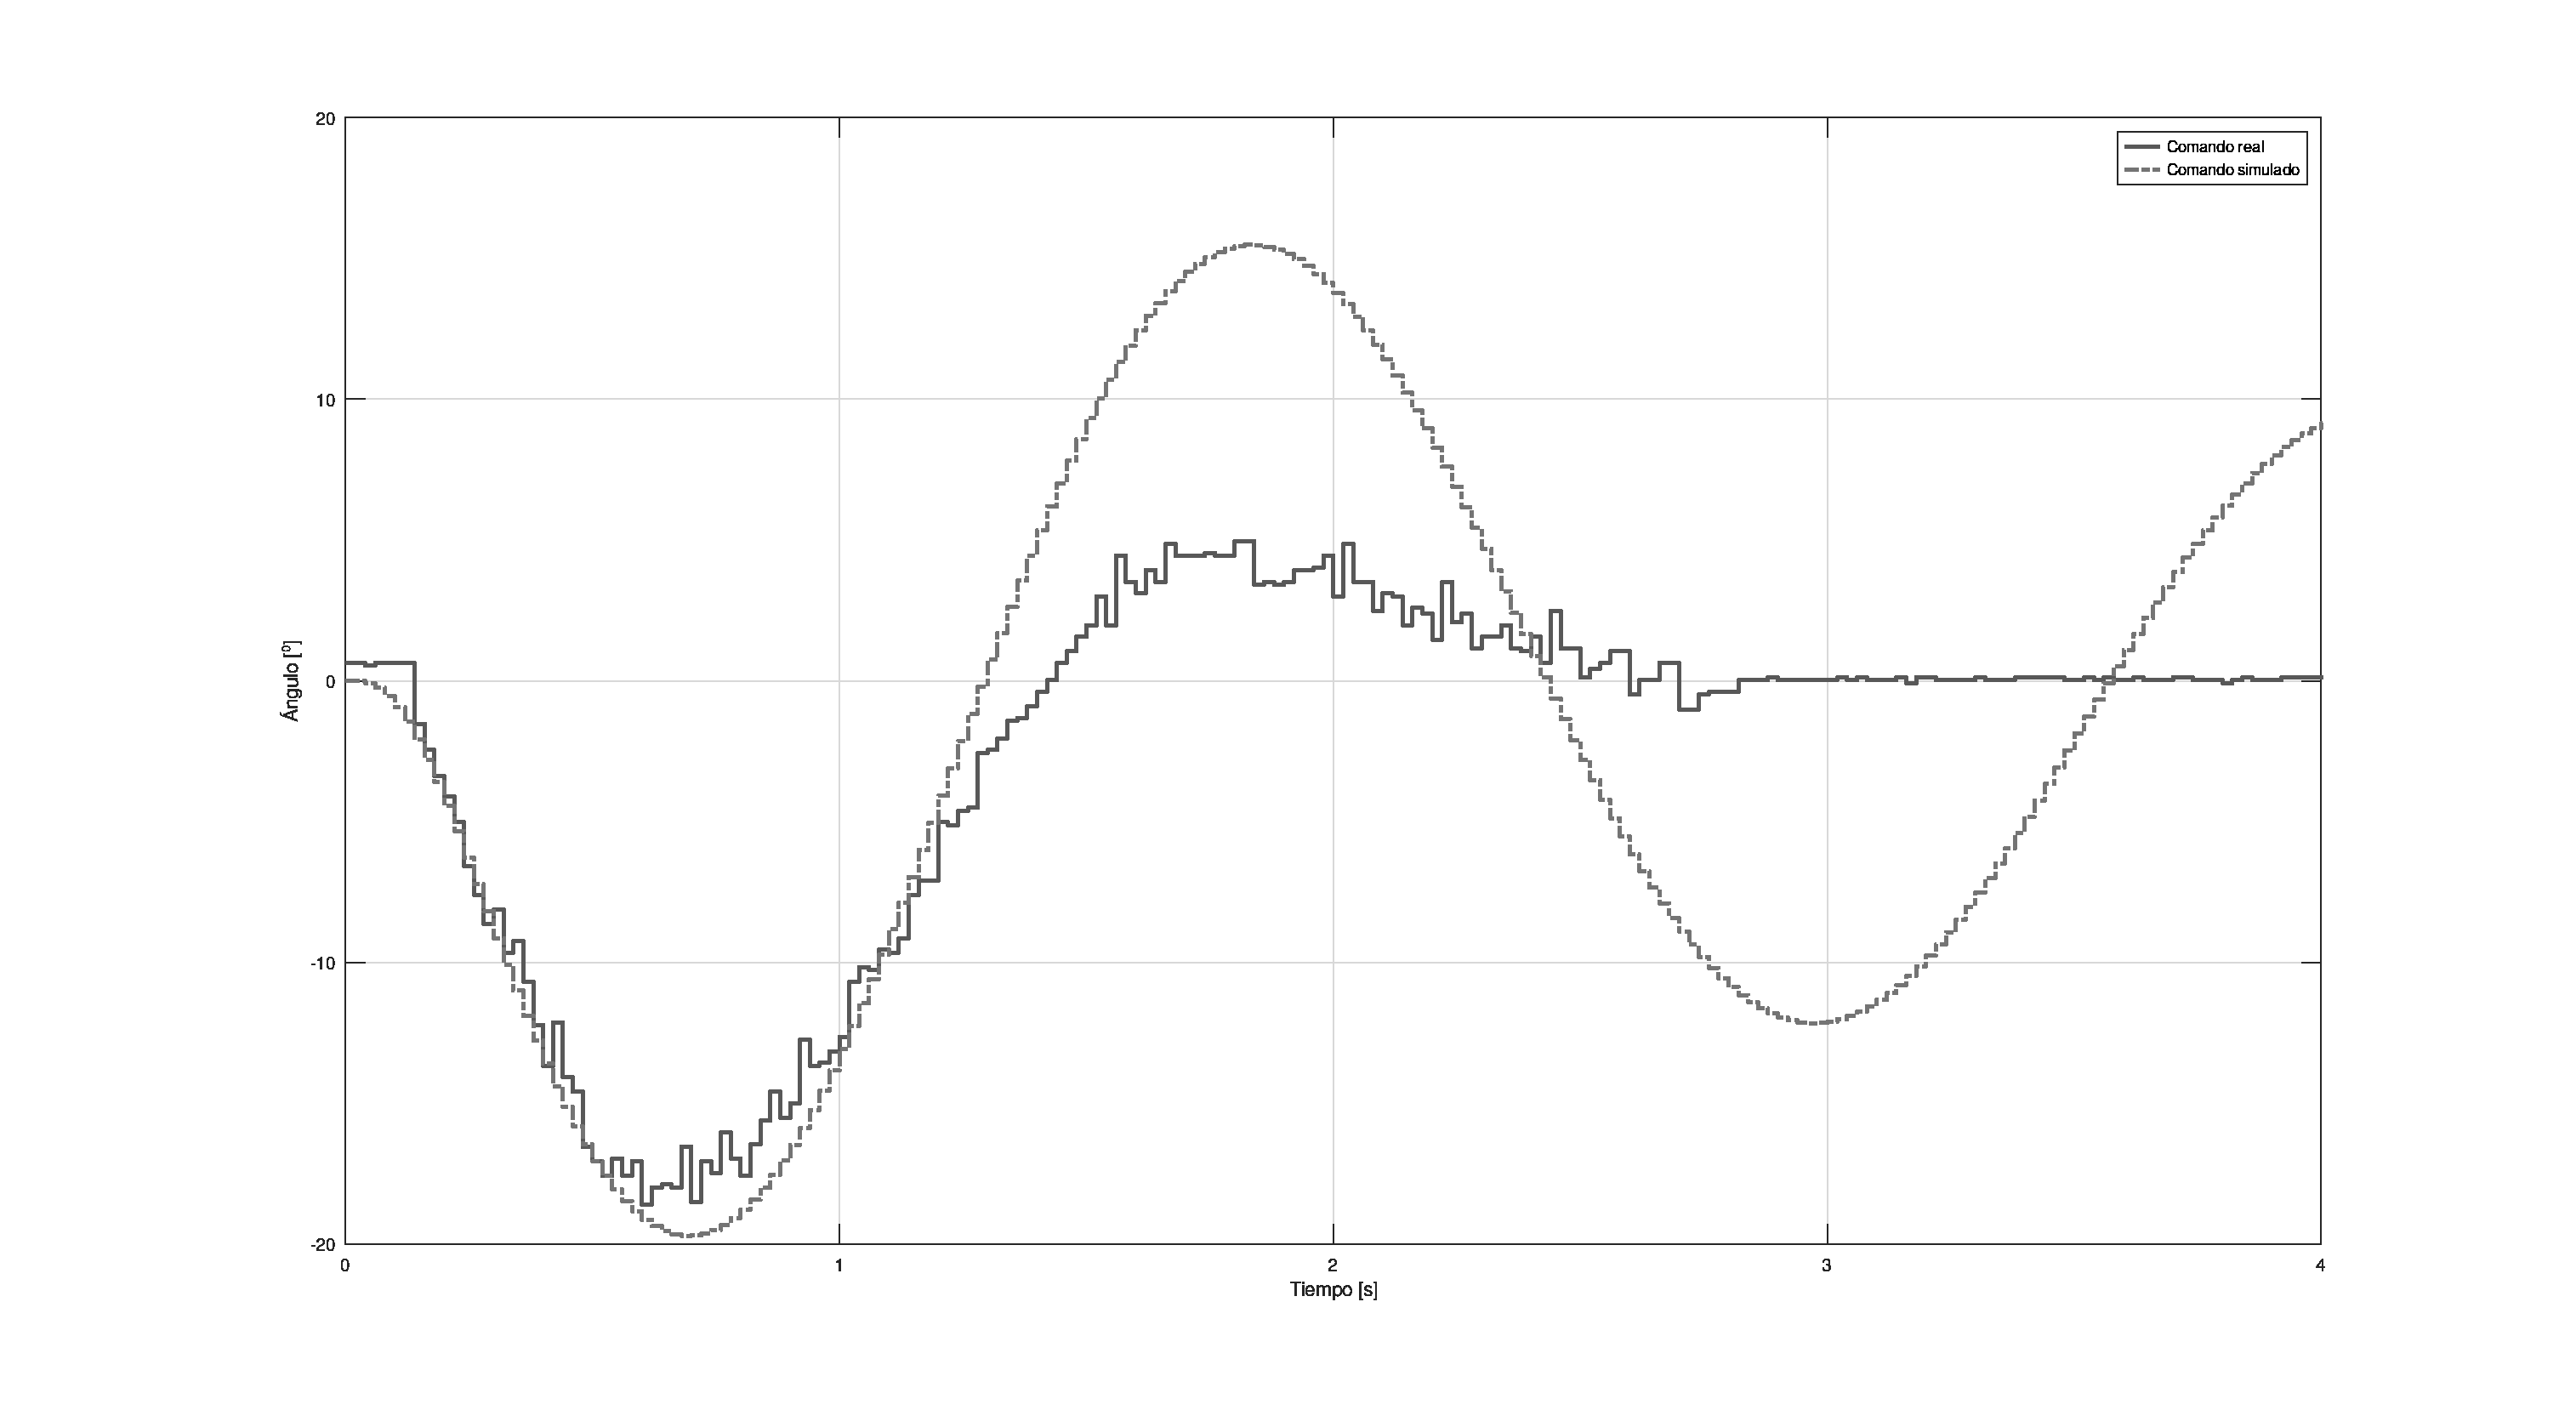
\includegraphics[width=\linewidth]{img/p-pert-cont.eps}
    \caption{Acción de control del sistema real y simulado ante una perturbación tipo impulso, y un lazo cerrado con un controlador tipo P.}
    \label{fig:p-pert-cont}
\end{figure}

\subsubsection{Respuesta al escalón de referencia}

La Figura~\ref{fig:p-ref-salida} muestra la salida de la planta ---la posición del carrito--- real y simulada, ante un escalón de referencia de \qty{0.1}{\m}, con el lazo cerrado por el controlador P.

Por la presencia del integrador en la planta, el controlador simulado eventualmente logra establecer a la planta en la referencia deseada. Sin embargo, producto de la fricción no modelada, el carrito en la realidad se frena. La posición medida no se establece en los \qty{0.1}{\m}, presentando un error no nulo en estado estacionario de aproximadamente un centímetro.

\begin{figure}[!tbp]
    \centering
    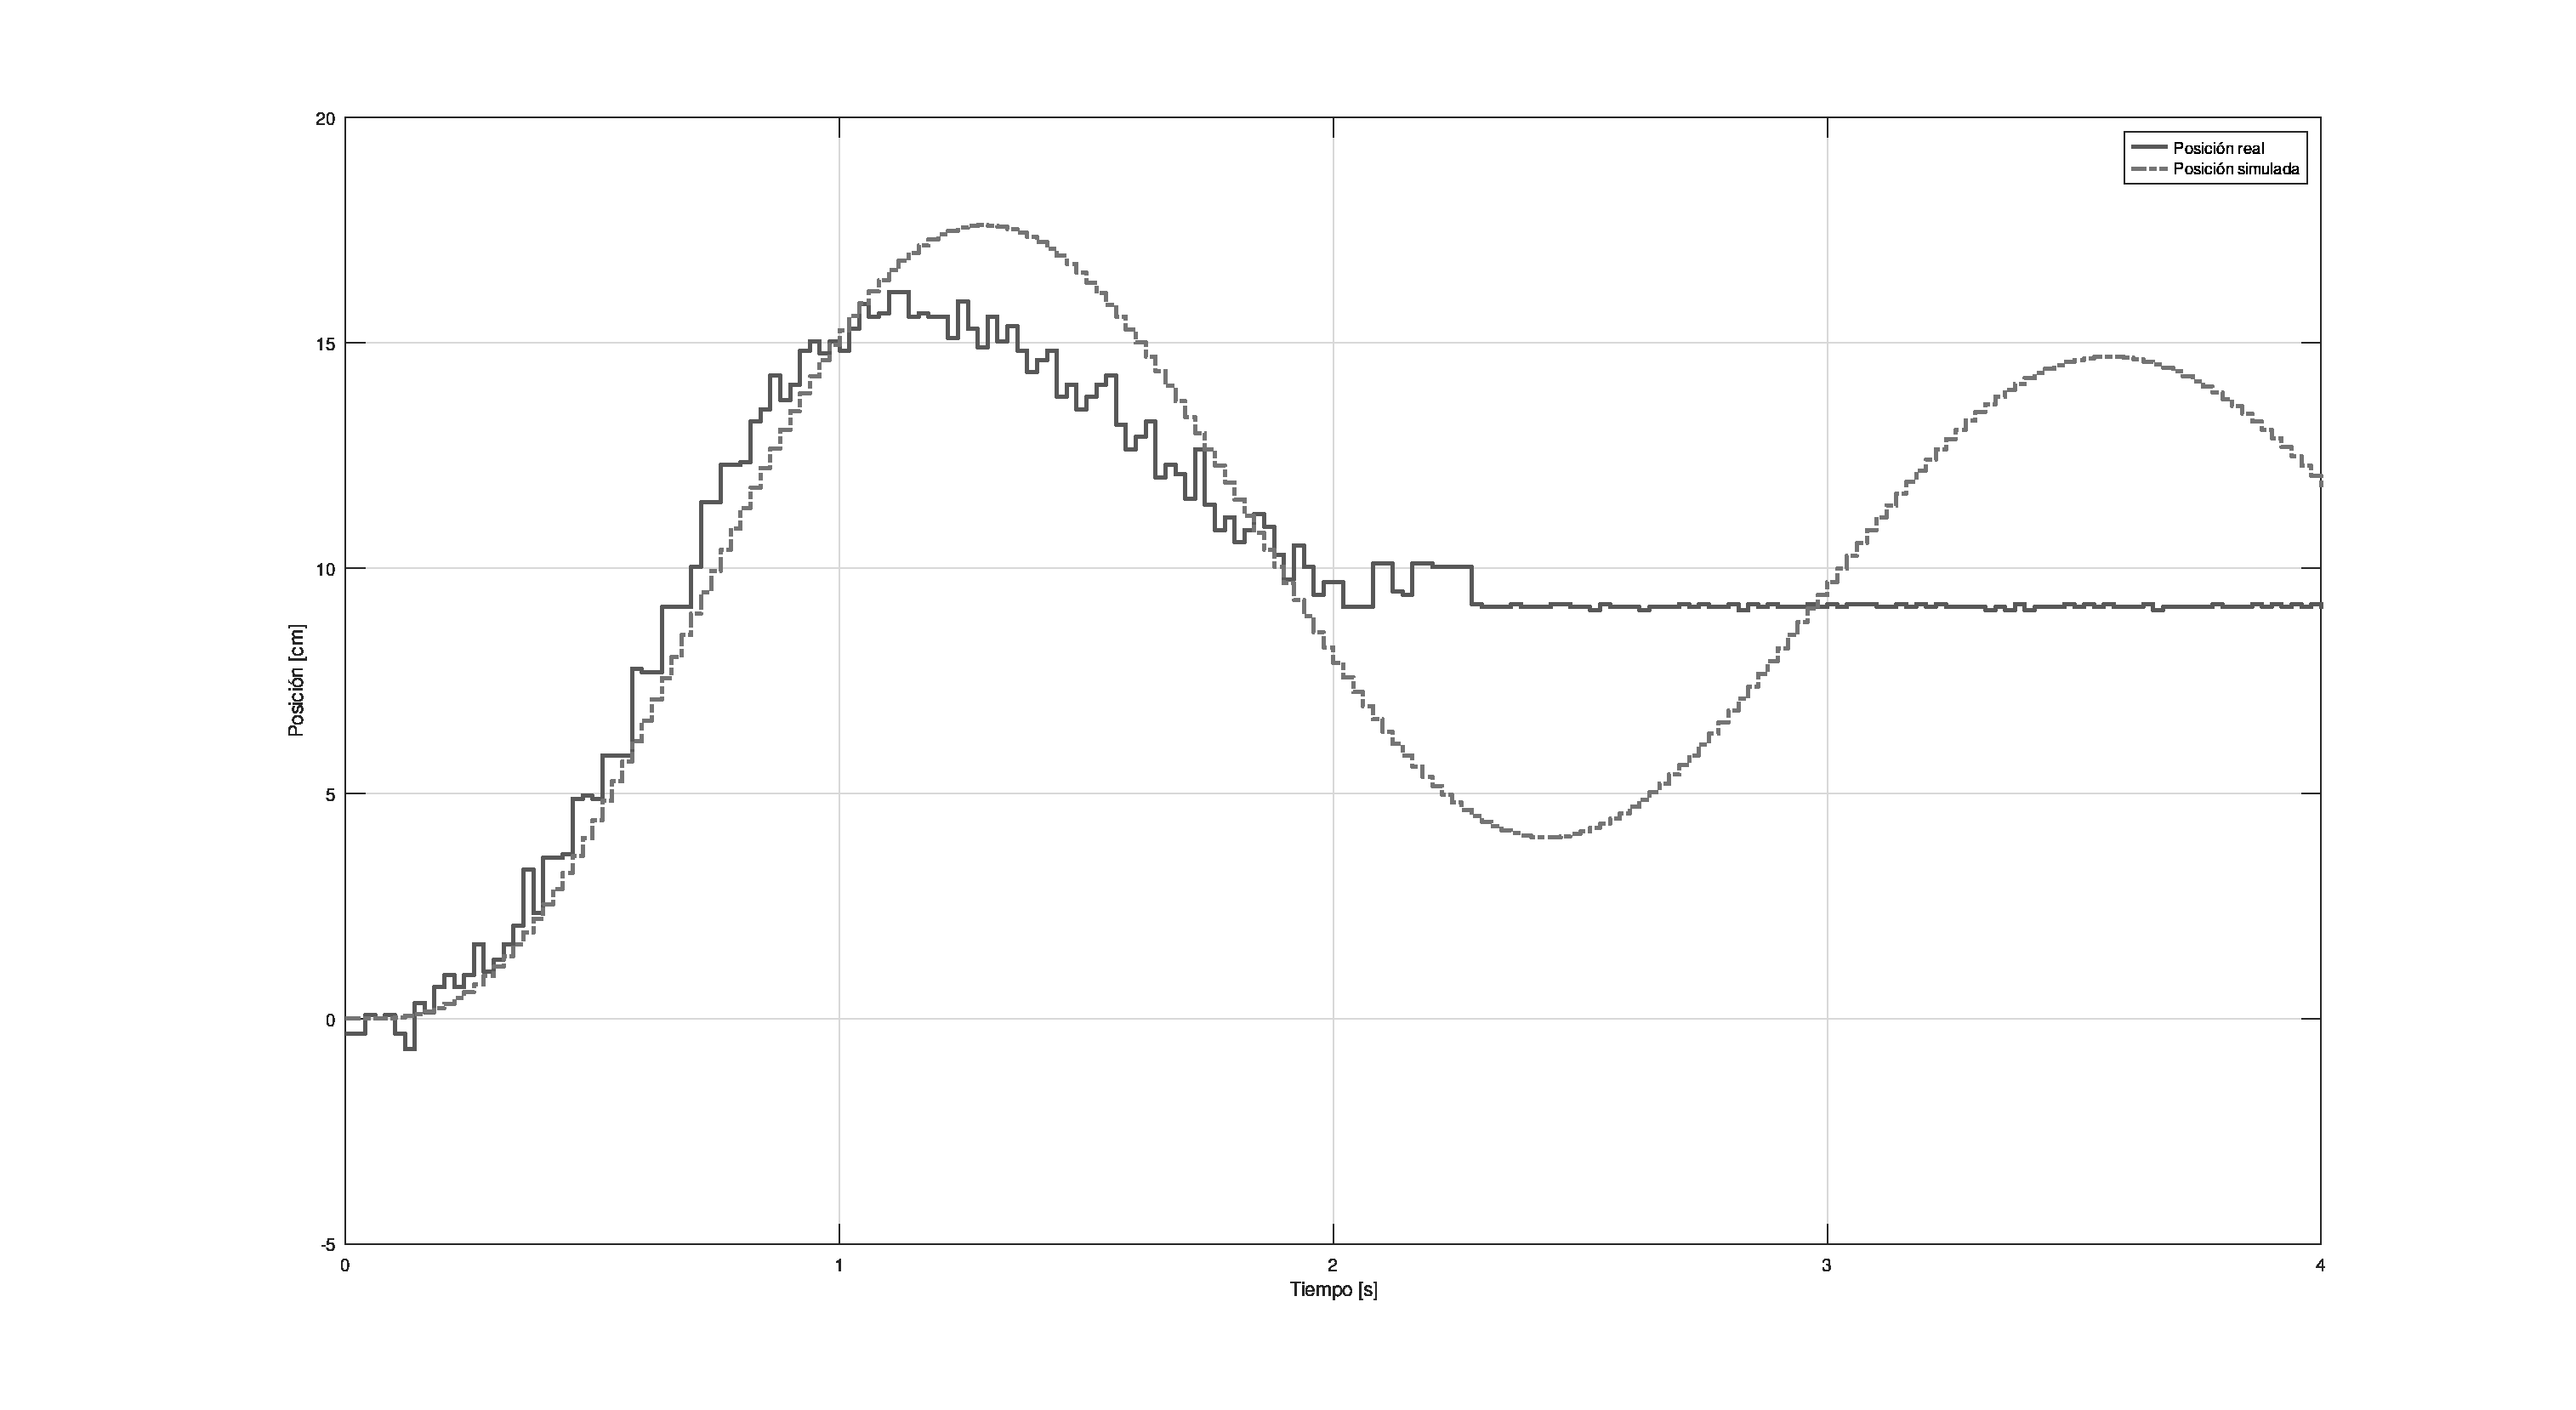
\includegraphics[width=\linewidth]{img/p-ref-salida.eps}
    \caption{Salida del sistema real y simulado ante un escalón de referencia, y un lazo cerrado con un controlador tipo P. Notar que las salidas se escalaron para estar en centímetros.}
    \label{fig:p-ref-salida}
\end{figure}

\subsection{Controlador PI}

El segundo control implementado fue un controlador proporcional-integral, para el cual se aplicaron las Ecuaciones~\eqref{eq:pid-u} y~\eqref{eq:pid-id}, utilizando
\begin{align*}
    K_p = -150, && K_i = -30, && K_d = 0.
\end{align*}

\subsubsection{Rechazo a perturbaciones tipo impulso}

La Figura~\ref{fig:pi-pert-salida} muestra la salida de la planta ---la posición del carrito--- real y simulada, ante una perturbación tipo impulso, con el lazo cerrado por el controlador PI y una referencia nula (punto de equilibrio).

Se observa que inicialmente hay una buena concordancia entre el modelo simulado y la planta real. Ambos sistemas presentan una oscilación de amplitudes similares, pero luego del segundo semiciclo la planta real se frena por el rozamiento. Esto produce un error en la posición final de unos \qty{4}{\cm}. Sin embargo, gracias a la acción integral, el carro puede volver a moverse a partir de los \qty{10}{\s}, para volver a frenarse, esta vez con un error mayor y de sentido contrario. A los \qty{13}{\s} vuelve a moverse, y se frena más cerca del cero. Un último movimiento cerca de los \qty{20}{\s} lleva el carro casi a la posición de equilibrio.

\begin{figure}[!tbp]
    \centering
    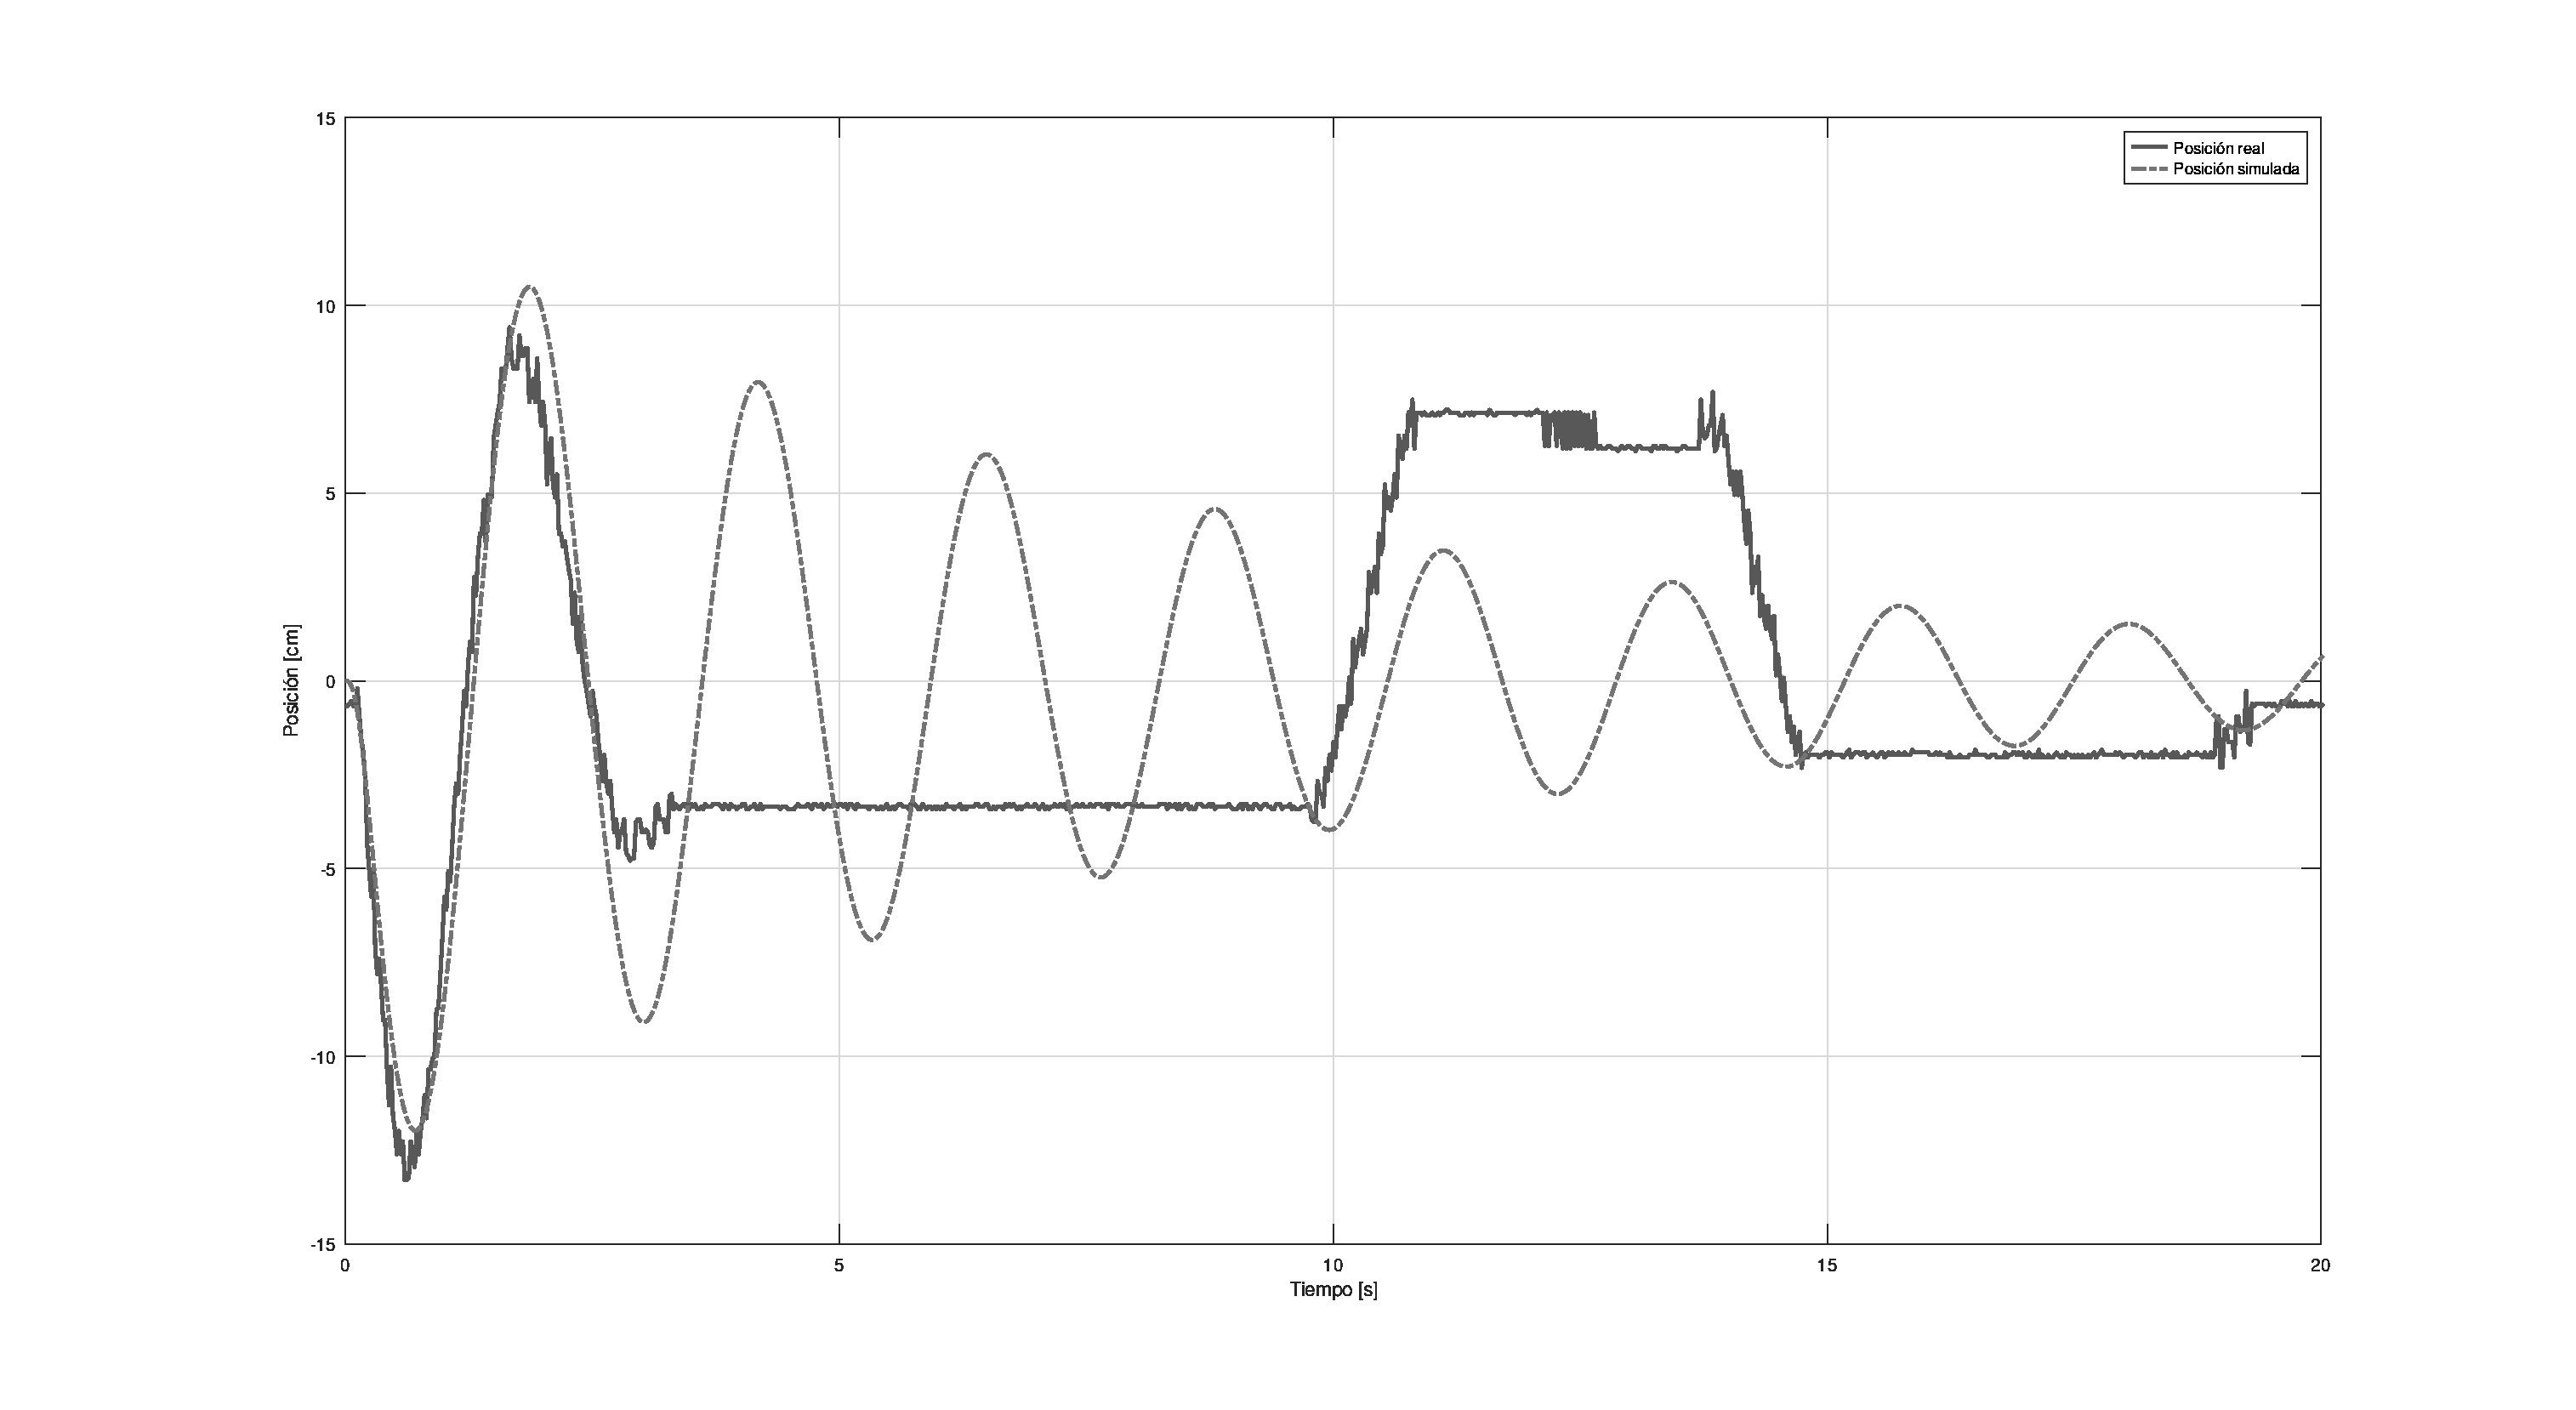
\includegraphics[width=\linewidth]{img/pi-pert-salida.eps}
    \caption{Salida del sistema real y simulado ante una perturbación tipo impulso, y un lazo cerrado con un controlador tipo PI. Notar que las salidas se escalaron para estar en centímetros.}
    \label{fig:pi-pert-salida}
\end{figure}

La Figura~\ref{fig:pi-pert-cont} muestra la acción de control ---el comando enviado al servomotor--- real y simulada, ante una perturbación tipo impulso, con el lazo cerrado por el controlador Pi y una referencia nula (punto de equilibrio). Observar que la acción de control en ningún caso satura los límites impuestos anteriormente. En este caso, vemos que cuando el carro se detiene, la acción de control sigue aumentando por la presencia de un error, gracias a la acción integral. Esto permite que el carro pueda volver a moverse tras quedar detenido por la fricción, reduciendo el error en estado estacionario.

\begin{figure}[!tbp]
    \centering
    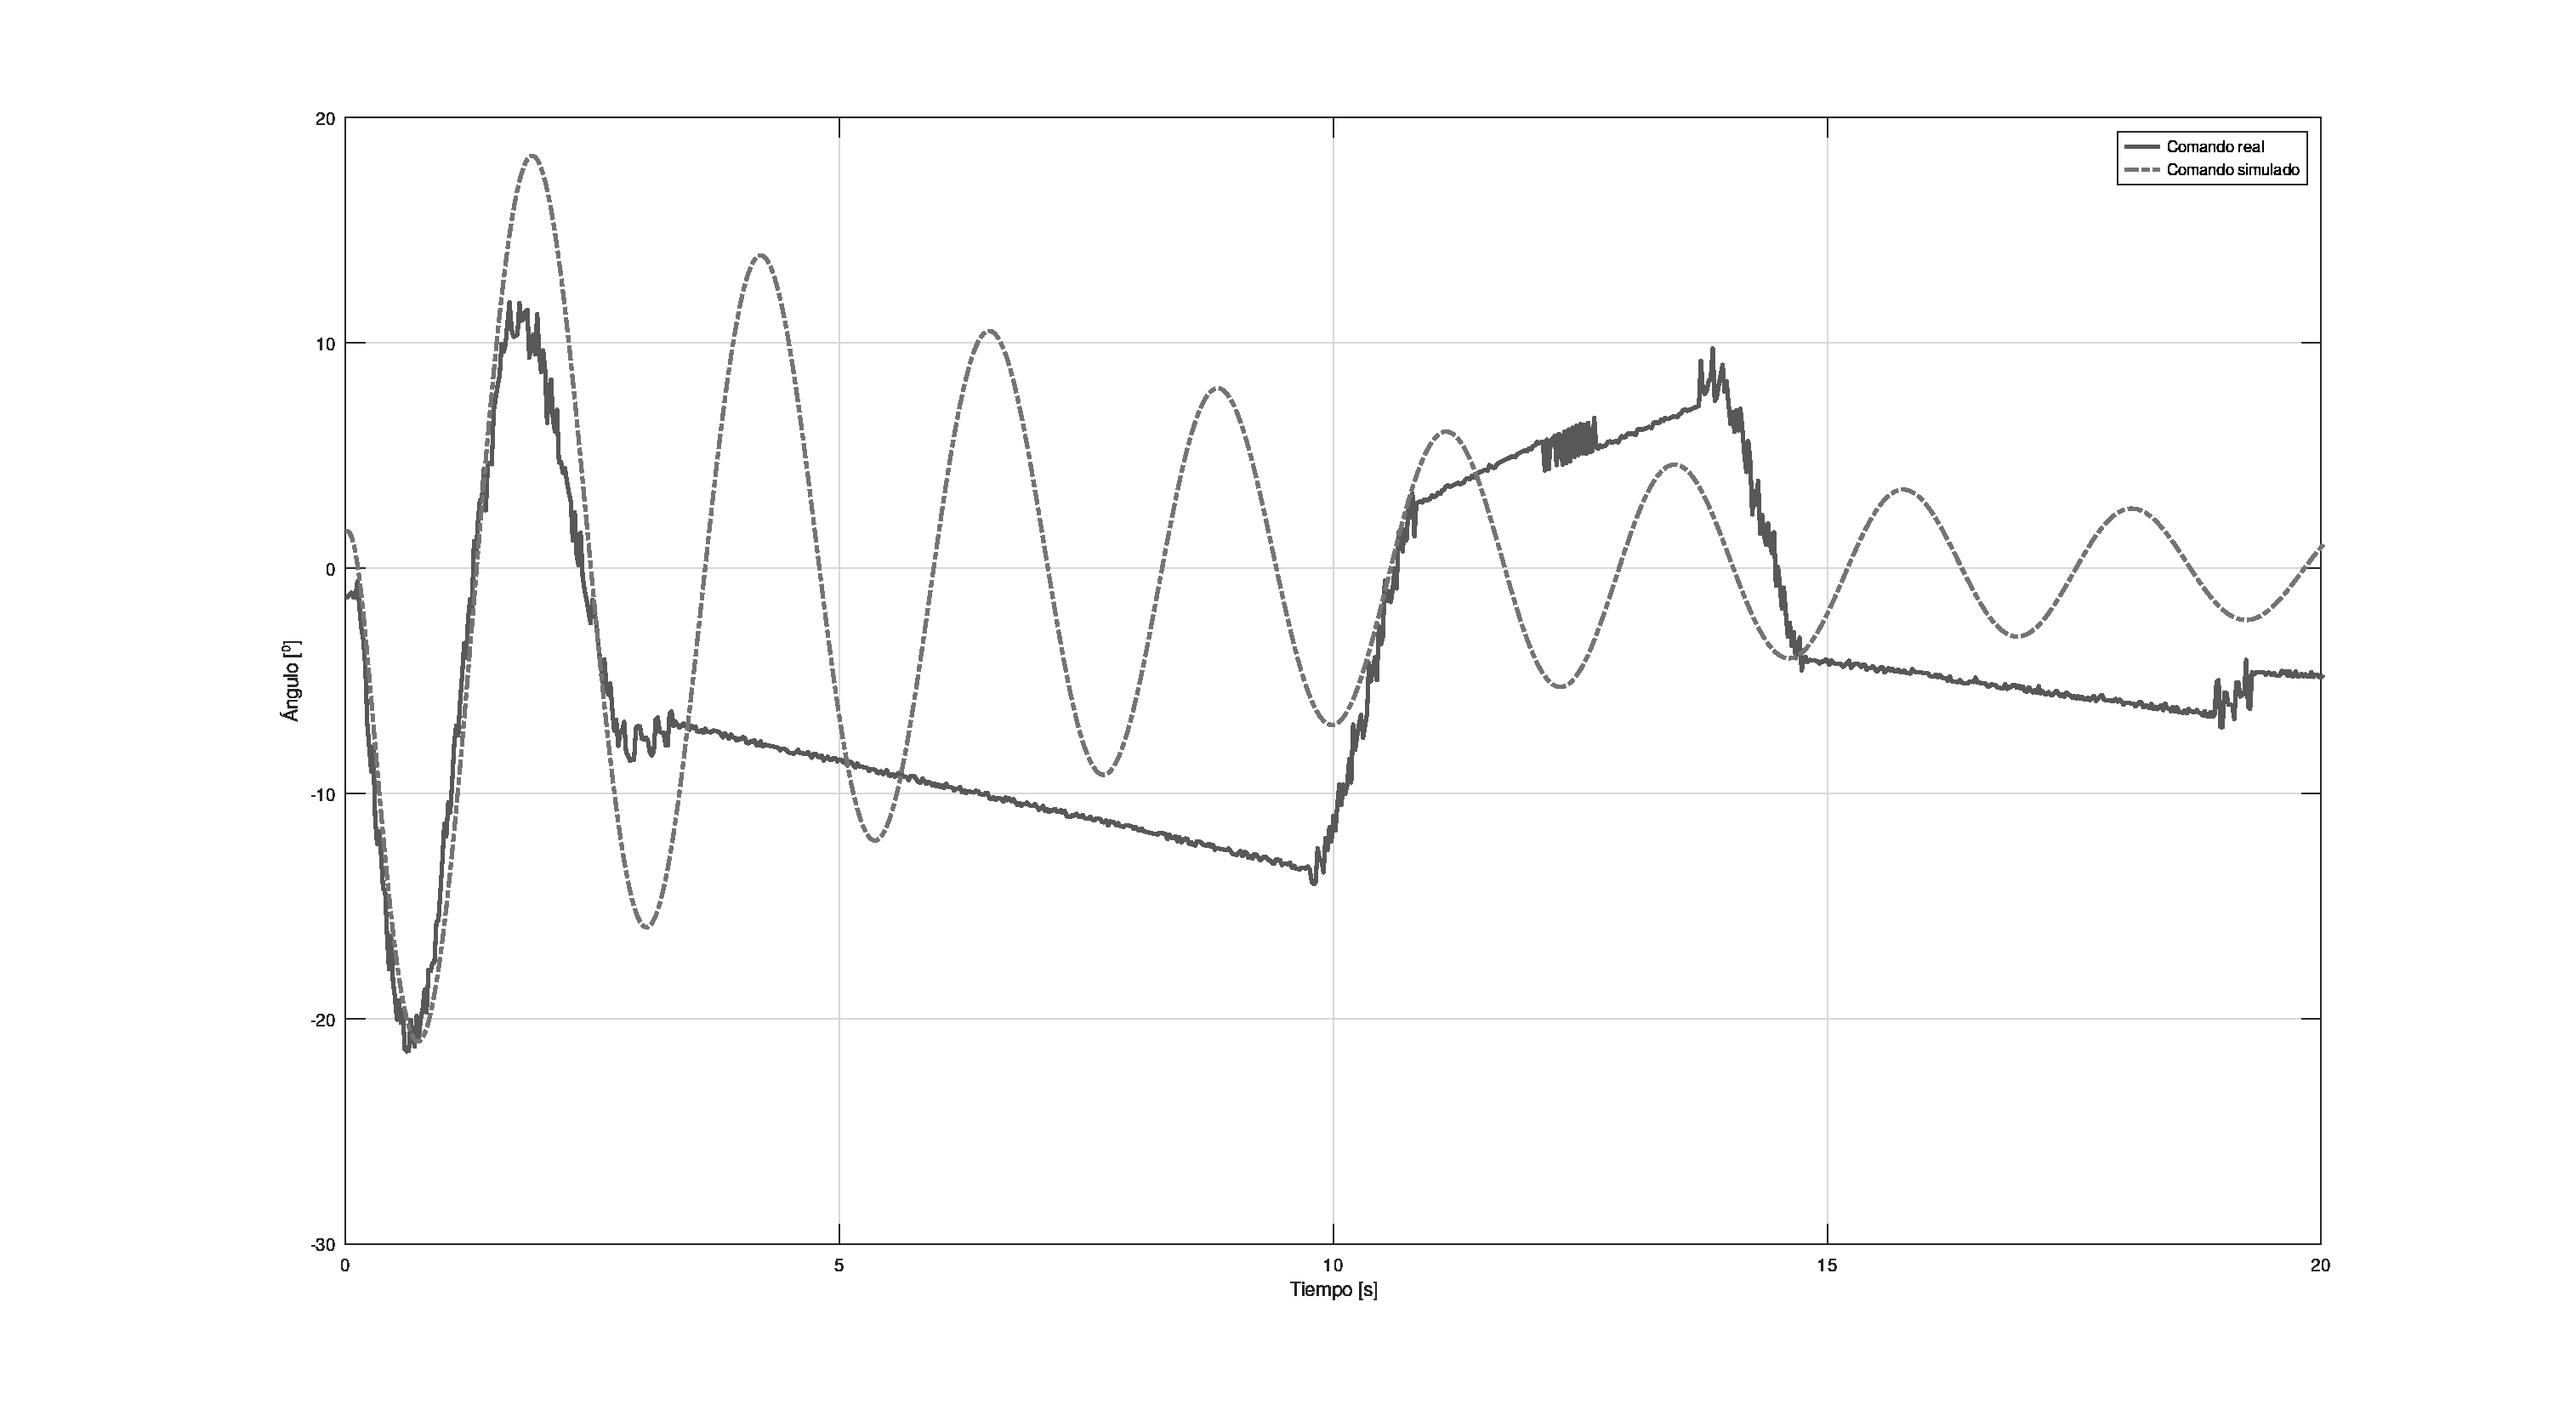
\includegraphics[width=\linewidth]{img/pi-pert-cont.eps}
    \caption{Acción de control del sistema real y simulado ante una perturbación tipo impulso, y un lazo cerrado con un controlador tipo PI.}
    \label{fig:pi-pert-cont}
\end{figure}

\subsubsection{Respuesta al escalón de referencia}

La Figura~\ref{fig:pi-ref-salida} muestra la salida de la planta ---la posición del carrito--- real y simulada, ante un escalón de referencia de \qty{0.1}{\m}, con el lazo cerrado por el controlador PI.

Inicialmente, la simulación y la planta real se comportan en forma similar. Una vez que el carro se detiene por la fricción, correcciones posteriores por la acción integral del controlador logran reducir el error en estado estacionario casi hasta cero, algo que no ocurría con el control P. La planta simulada eventualmente deja de oscilar y se establece exactamente en la referencia.

\begin{figure}[!tbp]
    \centering
    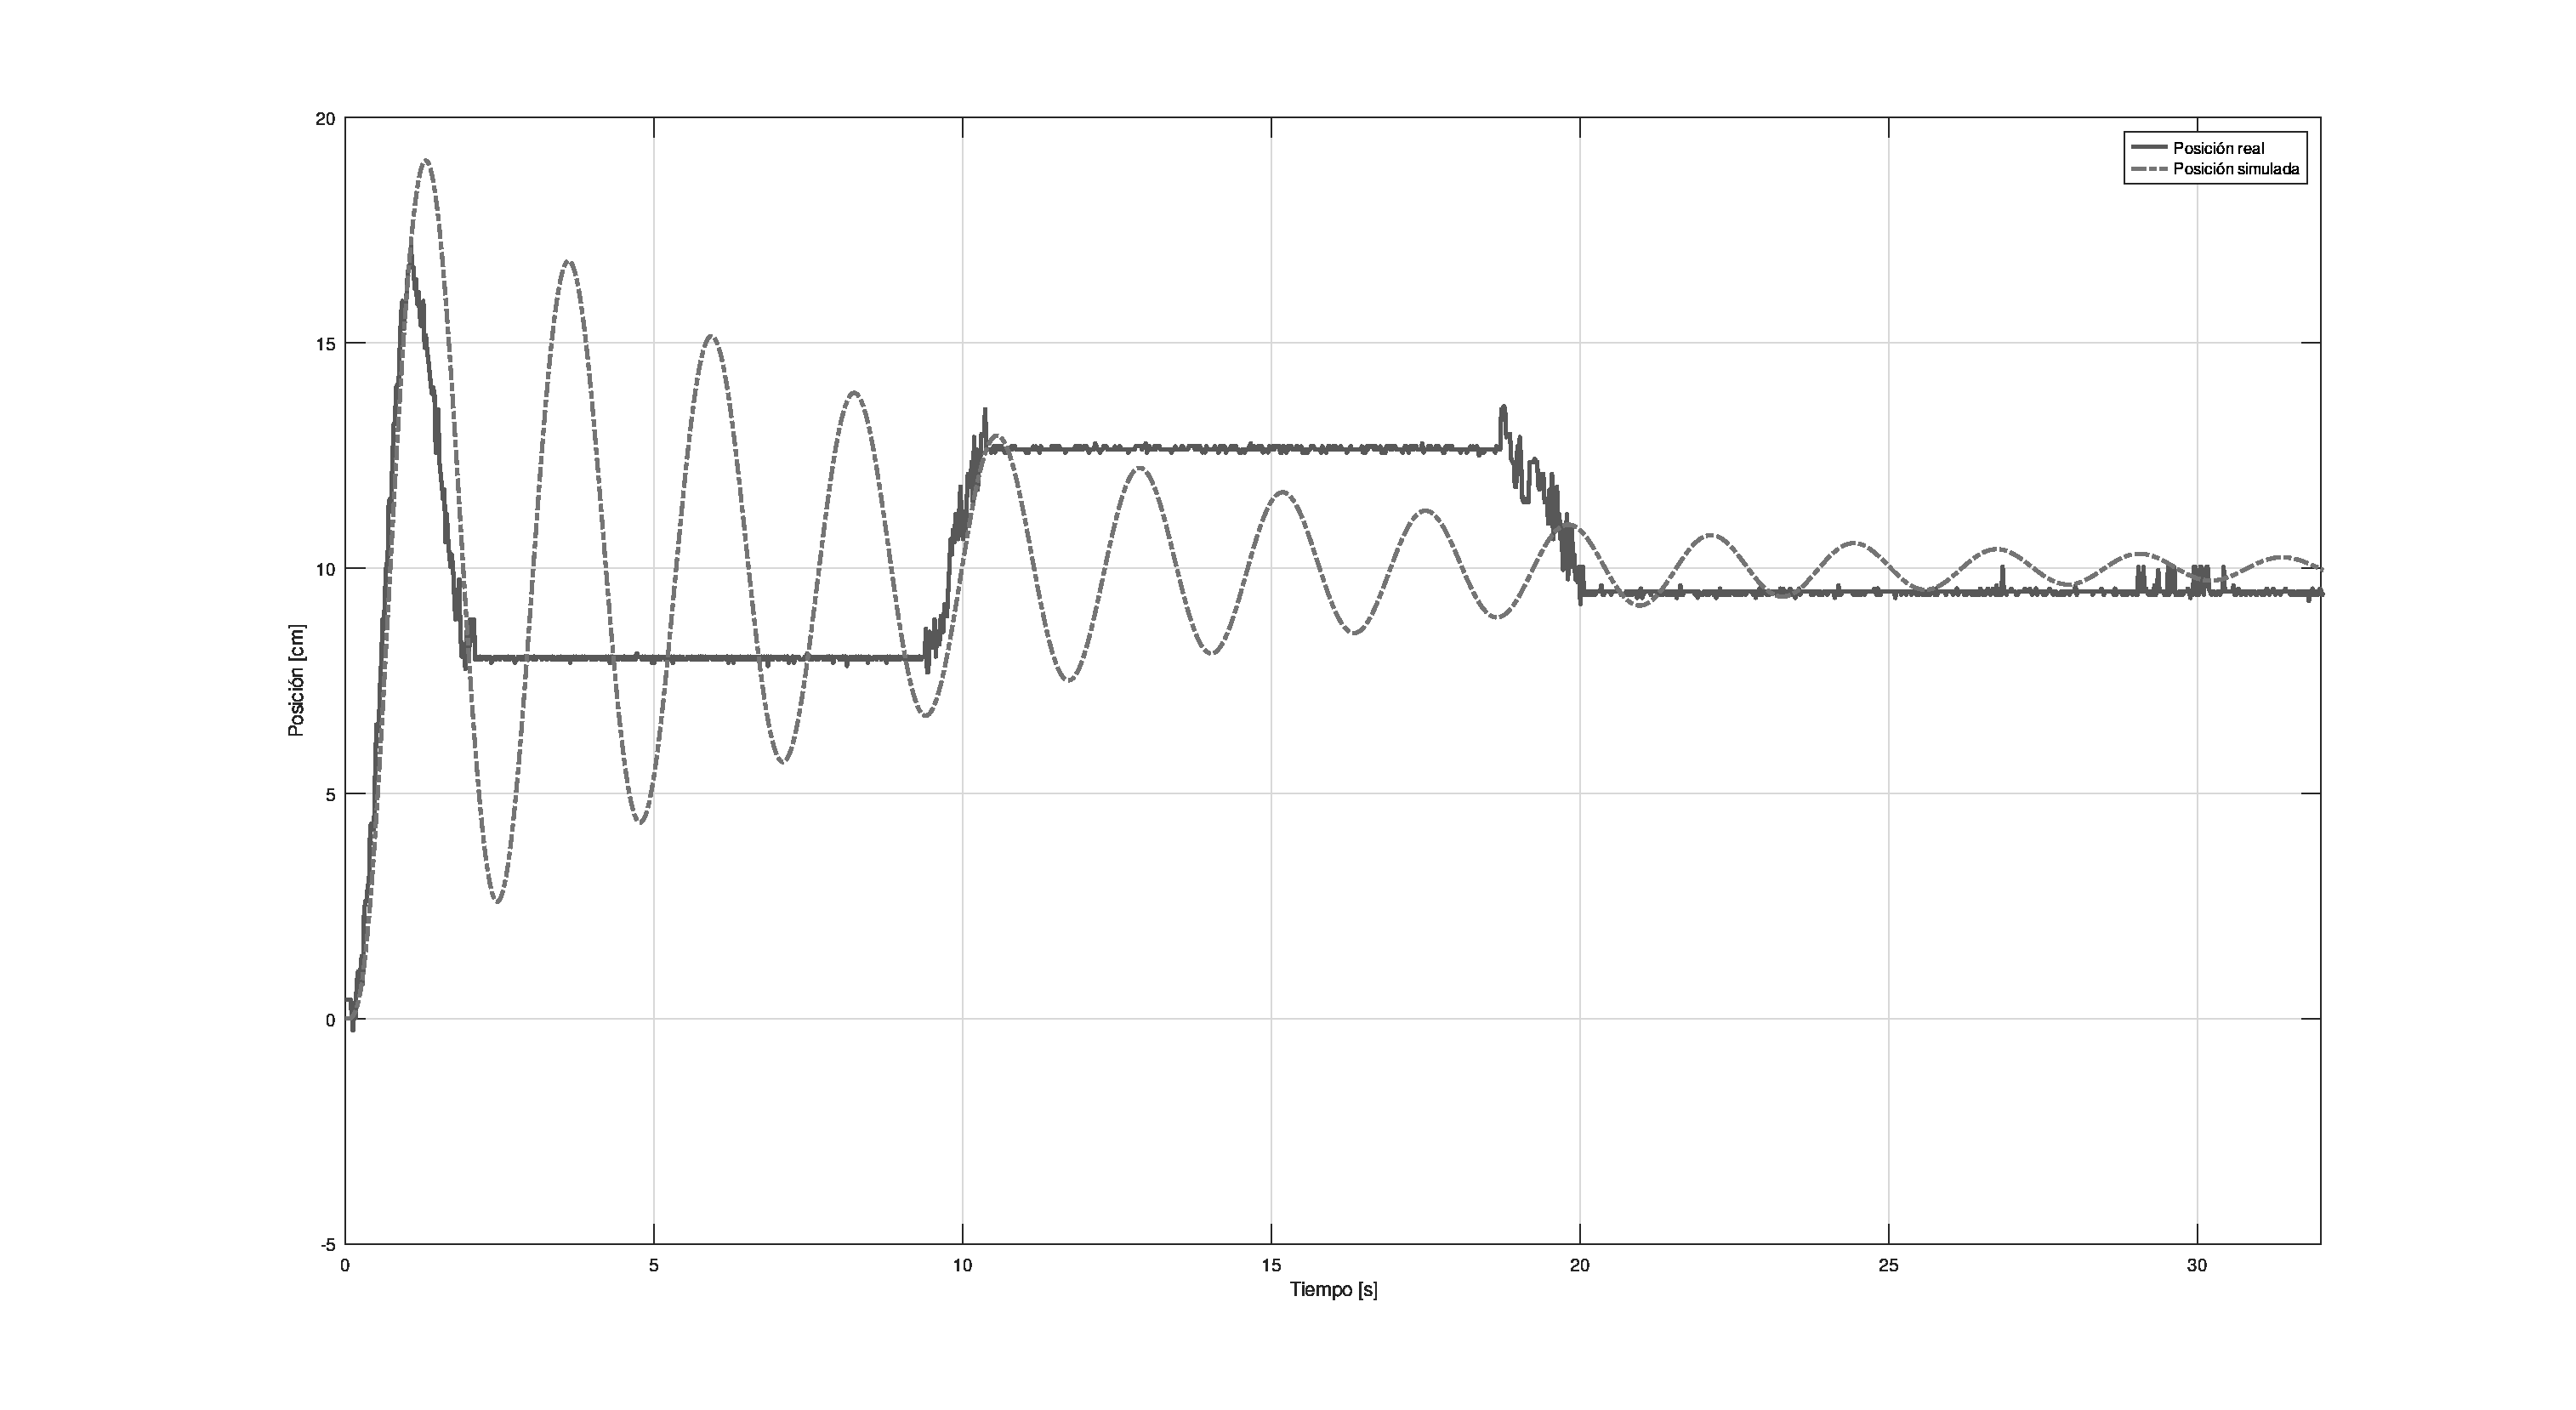
\includegraphics[width=\linewidth]{img/pi-ref-salida.eps}
    \caption{Salida del sistema real y simulado ante un escalón de referencia, y un lazo cerrado con un controlador tipo PI. Notar que las salidas se escalaron para estar en centímetros.}
    \label{fig:pi-ref-salida}
\end{figure}

\subsection{Controlador PD}

El tercer control implementado fue un controlador proporcional-derivativo, para el cual se aplicaron las Ecuaciones~\eqref{eq:pid-u} y~\eqref{eq:pid-id}, utilizando
\begin{align*}
    K_p = -150, && K_i = 0, && K_d = -0.01.
\end{align*}
La constante derivativa se eligió pequeña para evitar amplificar el ruido de medición. Si se utilizara un valor mayor, se producirían vibraciones en la acción de control que desetabilizarían la planta.

\subsubsection{Rechazo a perturbaciones tipo impulso}

La Figura~\ref{fig:pd-pert-salida} muestra la salida de la planta ---la posición del carrito--- real y simulada, ante una perturbación tipo impulso, con el lazo cerrado por el controlador PD y una referencia nula (punto de equilibrio).

Se observa que inicialmente hay una buena concordancia entre el modelo simulado y la planta real. Ambos sistemas presentan una oscilación, pero el carrito real se detiene por efecto de la fricción. Debido a la ausencia de acción integral en el controlador, hay un pequeño error en estado estacionario. Notar que el comportamiento es similar al del control P, debido a que la constante derivativa tiene un valor bajo.

\begin{figure}[!tbp]
    \centering
    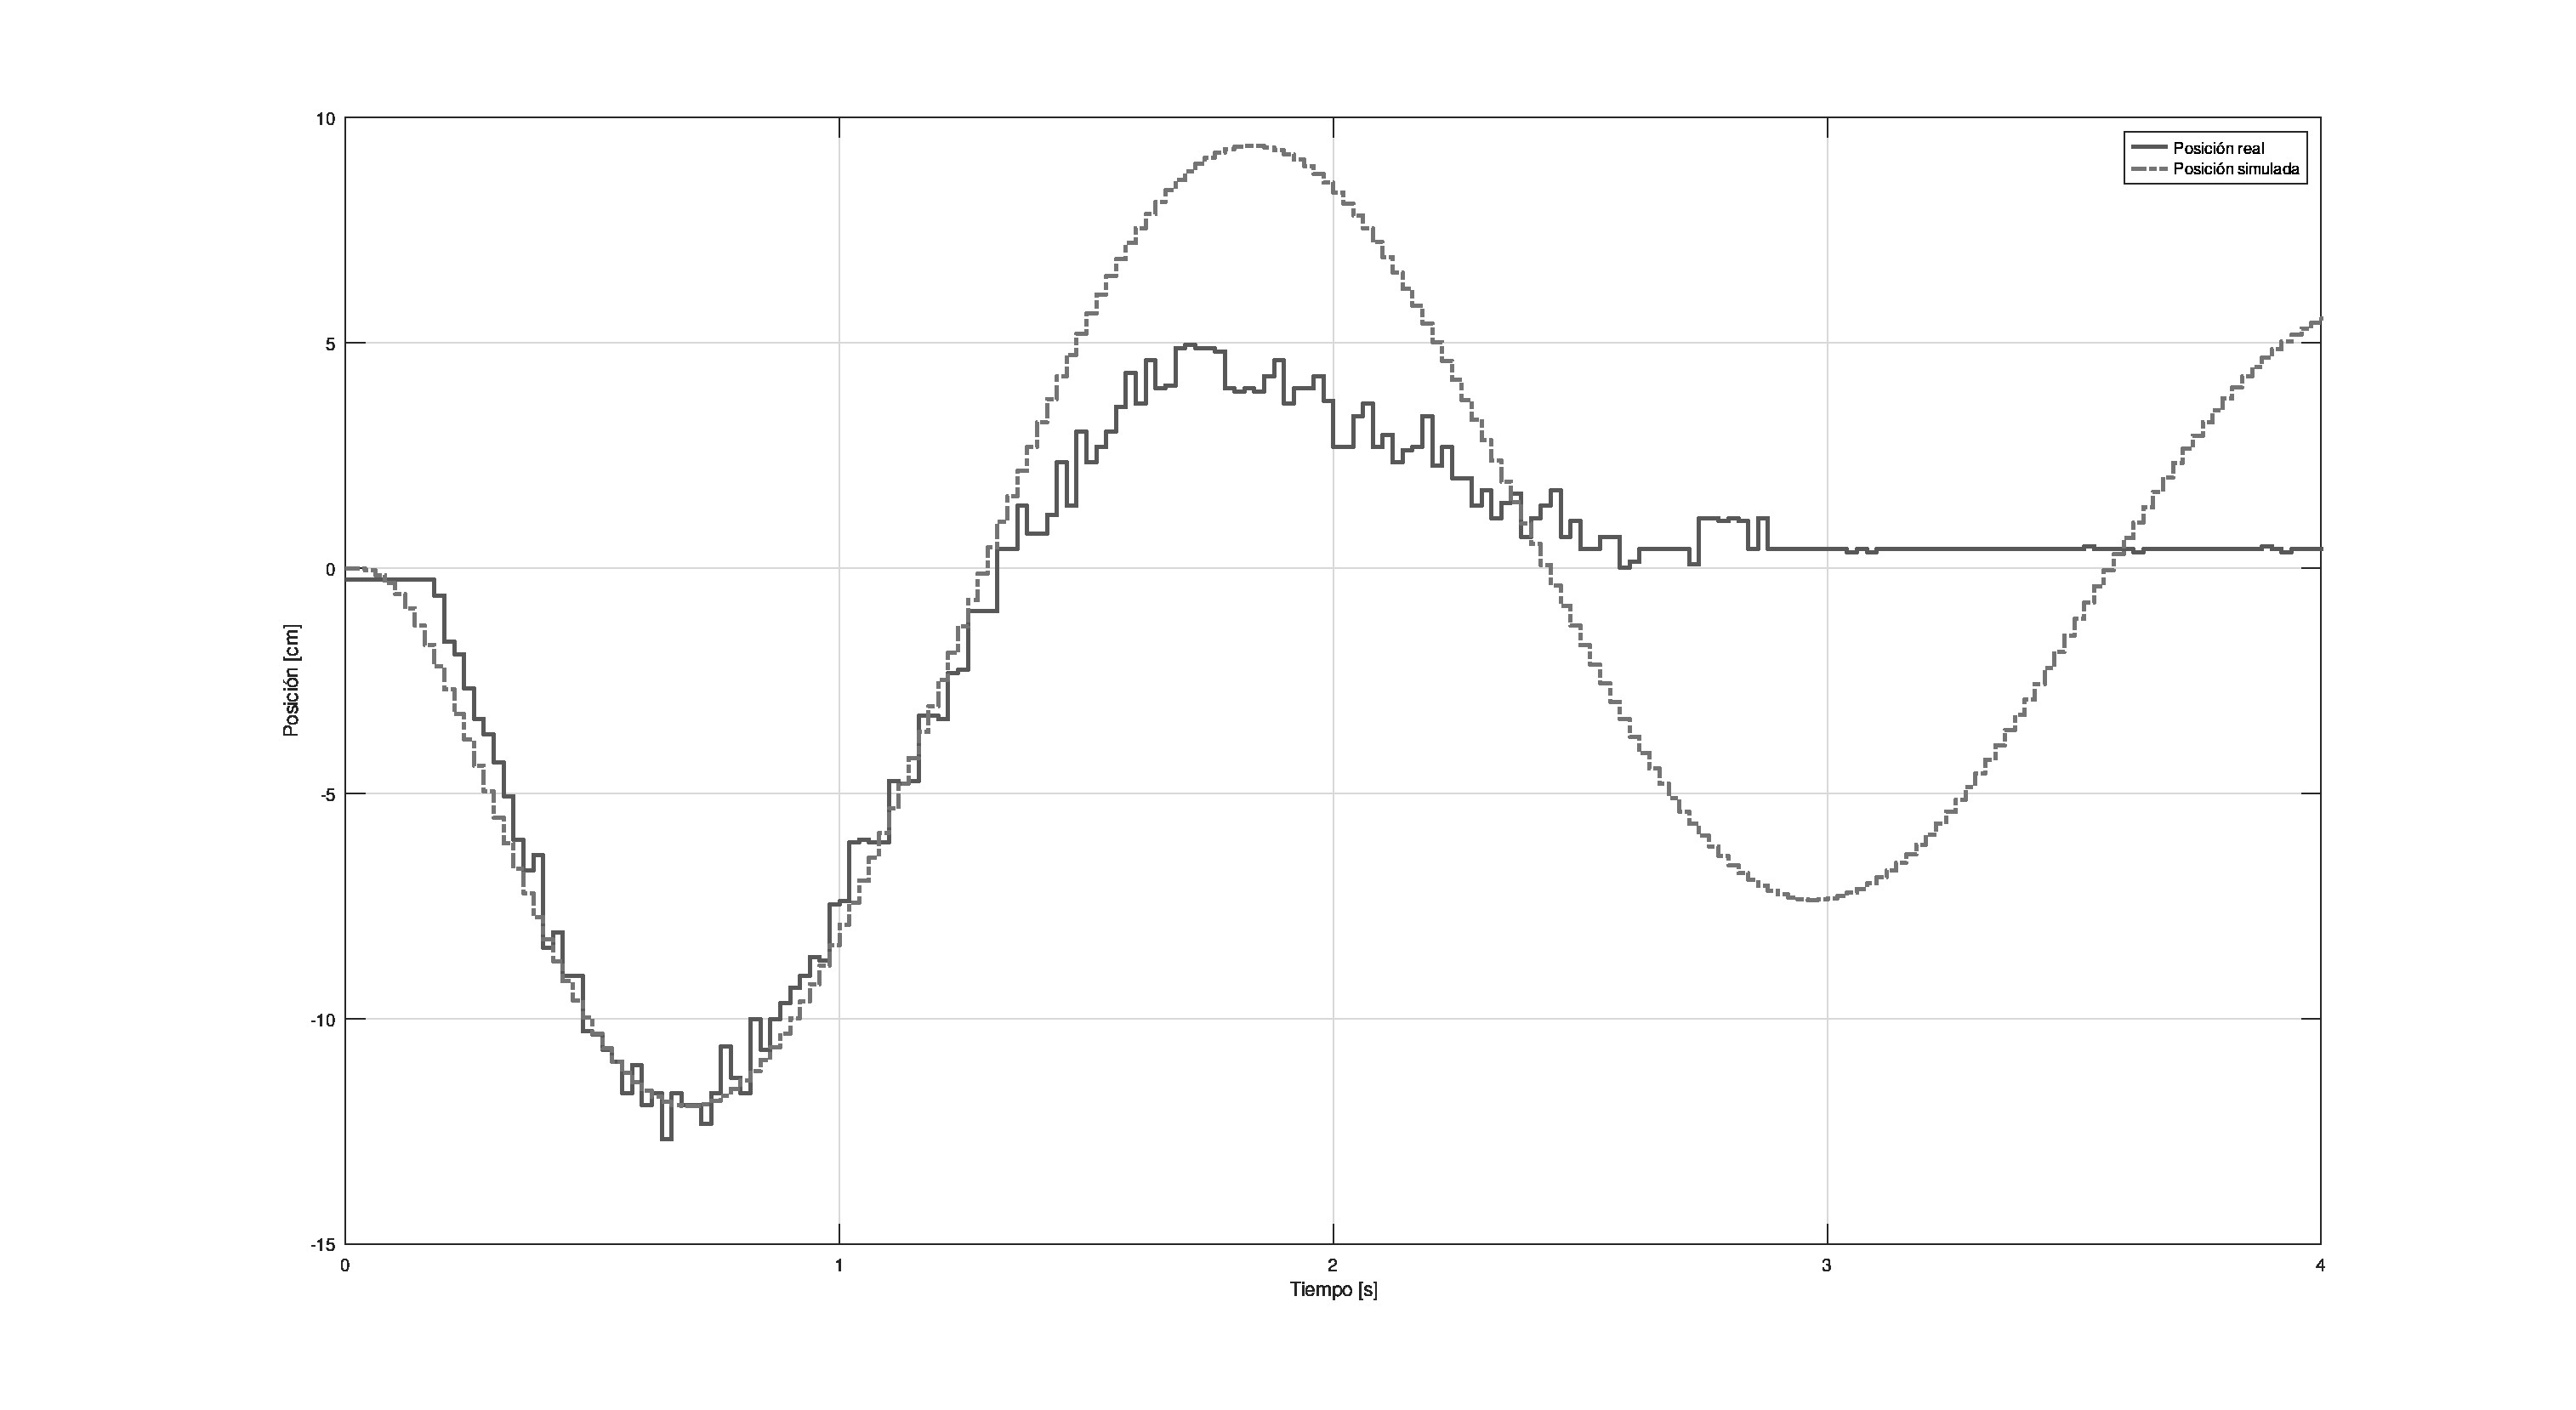
\includegraphics[width=\linewidth]{img/pd-pert-salida.eps}
    \caption{Salida del sistema real y simulado ante una perturbación tipo impulso, y un lazo cerrado con un controlador tipo PD. Notar que las salidas se escalaron para estar en centímetros.}
    \label{fig:pd-pert-salida}
\end{figure}

La Figura~\ref{fig:pd-pert-cont} muestra la acción de control ---el comando enviado al servomotor--- real y simulada, ante una perturbación tipo impulso, con el lazo cerrado por el controlador PD y una referencia nula (punto de equilibrio). Observar que la acción de control en ningún caso satura los límites impuestos anteriormente. En este caso, vemos que cuando el carrito se encuentra detenido, la acción de control presenta unas pequeñas oscilaciones producto de la amplificación del ruido. Este es el problema encontrado con el controlador PD. Si se usara una constante derivativa mayor, esas vibraciones producirían la caída del carrito o la inestabilización del sistema.

\begin{figure}[!tbp]
    \centering
    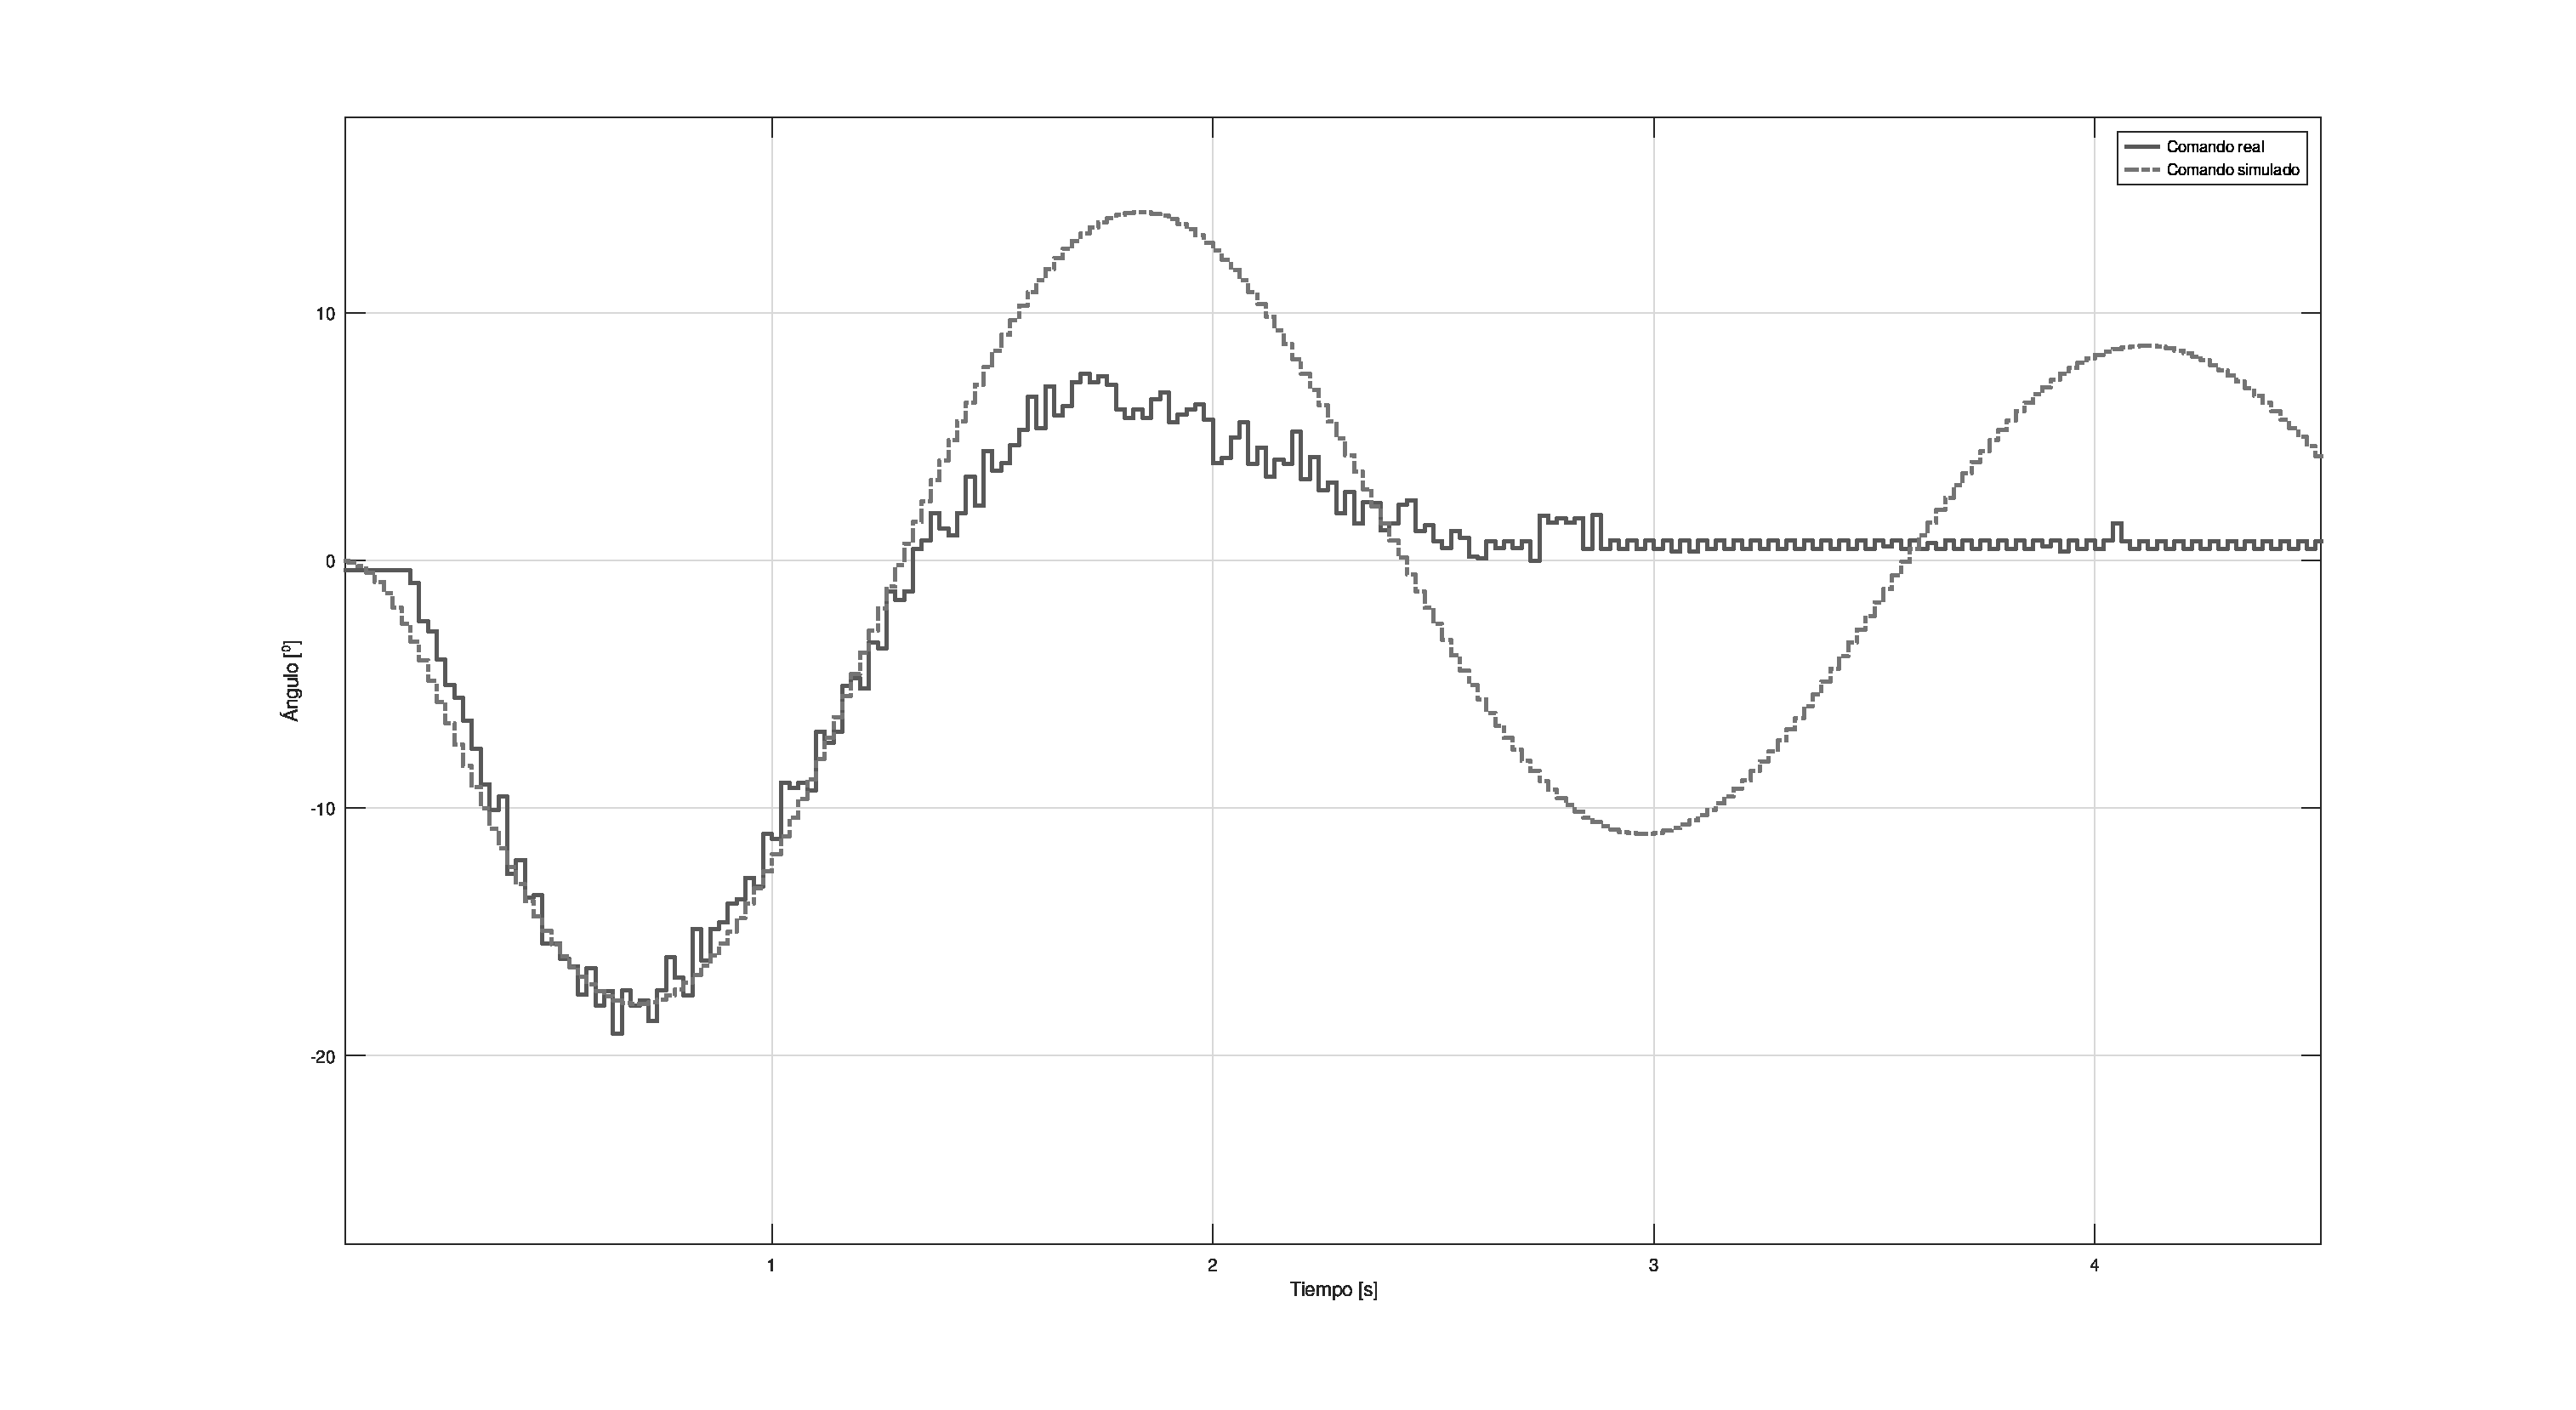
\includegraphics[width=\linewidth]{img/pd-pert-cont.eps}
    \caption{Acción de control del sistema real y simulado ante una perturbación tipo impulso, y un lazo cerrado con un controlador tipo PD.}
    \label{fig:pd-pert-cont}
\end{figure}

\subsubsection{Respuesta al escalón de referencia}

La Figura~\ref{fig:pd-ref-salida} muestra la salida de la planta ---la posición del carrito--- real y simulada, ante un escalón de referencia de \qty{0.1}{\m}, con el lazo cerrado por el controlador PD.

Inicialmente, hay una muy buena concordancia entre el sistema real y el simulado. Sin embargo, por efecto de la fricción no modelada, el carrito real se frena, mientras que la simulación continúa oscilando durante un tiempo más. Además, hay un error no nulo en estado estacionario, ya que la ausencia de acción integral en el controlador imposibilita corregir una vez que el carro se atascó. La acción derivativa no tiene un gran efecto porque la constante elegida es baja.

\begin{figure}[!tbp]
    \centering
    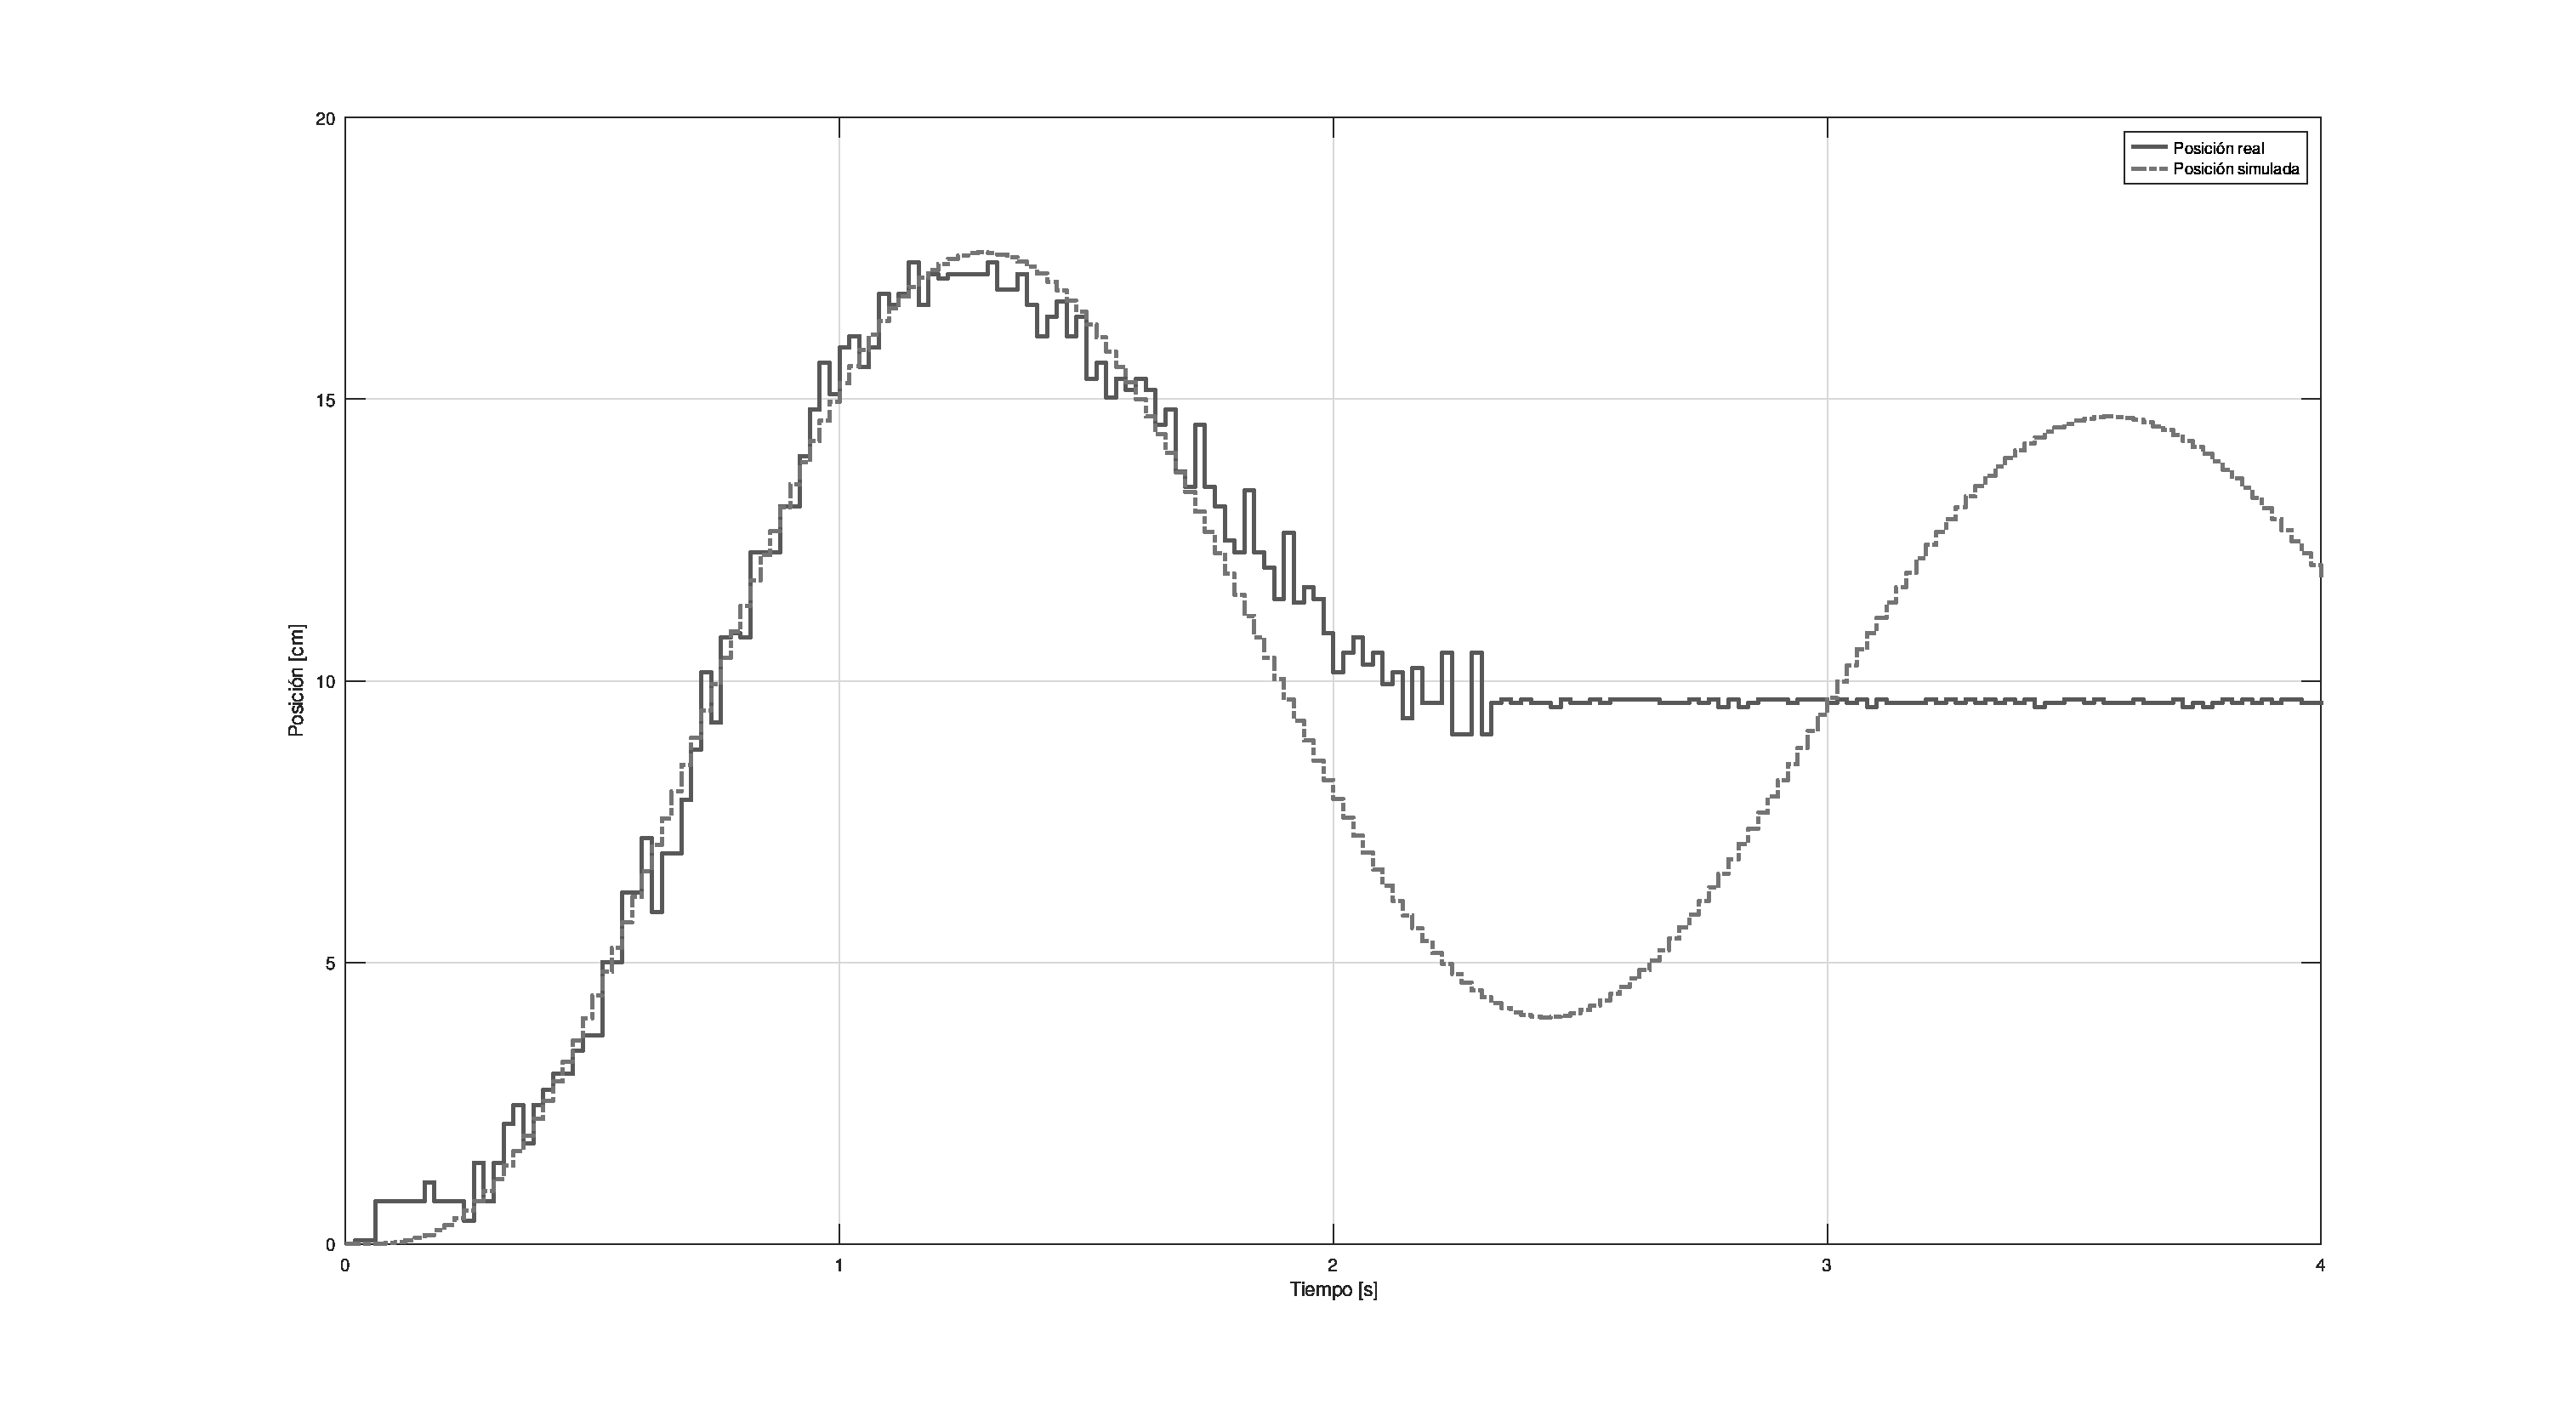
\includegraphics[width=\linewidth]{img/pd-ref-salida.eps}
    \caption{Salida del sistema real y simulado ante un escalón de referencia, y un lazo cerrado con un controlador tipo PD. Notar que las salidas se escalaron para estar en centímetros.}
    \label{fig:pd-ref-salida}
\end{figure}

% vim: ts=4 sts=4 sw=4 et lbr
